\chapter{REFERENCIAL TEÓRICO}
\onehalfspacing
Nesse item serão apresentados conceitos primordiais para compreensão da presente pesquisa. 

\section{CICLO HIDROLÓGICO}

Para que se chegue ao entendimento de um assunto, faz-se necessária a compreensão de tudo aquilo que o toca em seu entorno, e com as chuvas intensas não é diferente. Assim sendo, é notório que as primeiras noções precisam ser acerca do elemento que rege todo o tema, que é a água, além da ciência que busca conhecer a sua relação com o objeto de estudo.

A água é o elemento mais importante e comum no planeta Terra. Sendo essencial à existência, está presente de diferentes formas na vida dos seres. Ela pode ser encontrada em três formas físicas diferentes, a sólida, a líquida e a gasosa. 

A ciência que estuda a água na Terra é a hidrologia. Segundo Wisler e Brater (1959), ela trata dos processos que guiam o reabastecimento e perda de água sobre o mar, do transporte dela através do ar, da terra, sobre e abaixo de sua superfície. Em suma, ela trata das várias partes do ciclo hidrológico. Collischonn e Dornelles (2015) entendem que suas áreas de conhecimento percorrem à hidráulica, física e estatística, que por sua vez são utilizados na descrição dos mecanismos do ciclo da água, e compreensão de suas variáveis.

Collischonn e Dornelles (2015) ainda mencionam que o que diferencia a Hidrologia das outras ciências que almejam compreender como a água se comporta, é a dedicação principal à busca do entendimento dos processos do ciclo hidrológico em contato com os continentes, de forma a tentar responder o que ocorre com a água da precipitação.

Porém, por mais que a hidrologia busque principalmente respostas a respeito da água precipitada, é importante entender que para o ciclo deste elemento, a precipitação é apenas um dos processos que ele engloba. Silveira (2012) descreve o ciclo hidrológico como um fenômeno global fechado. Este que impulsionado pela energia do sol junto à gravidade e rotação da Terra, permite a circulação da água por entre a superfície terrestre que envolve os continentes, oceanos e a atmosfera com suas diferentes camadas, em especial a troposfera, onde acontece grande parte dos fenômenos meteorológicos.

Silveira (2012) ainda explica os sentidos qual ocorrem as circulações do ciclo hidrológico, sendo eles divididos em dois. Um no sentido superfície-atmosfera, onde através de fenômenos como a evaporação e transpiração das plantas, é determinado o fluxo fundamentalmente na forma de vapor. O outro ocorre no sentido oposto, sendo ele atmosfera-superfície, onde a transferência da água se dá em qualquer um dos estados físicos, com as principais precipitações sendo de neve e chuva.

\newpage

A água quando precipitada, grande parte atinge o mar, sendo uma pequena parte evaporada antes mesmo de chegar ao chão, ou transpirada pelas plantas. Da parte que atinge o terreno uma parcela escoa da superfície e atinge estagnações ou cursos d'água, podendo ser rios ou bacias hidrográficas. Uma parte também infiltra no terreno, ficando armazenada na zona subterrânea da Terra, em lençóis freáticos por exemplo, ou escoando para outros cursos. De forma simplificada, grande parte dessa água retorna à atmosfera através da evaporação. Wilken (1978) resume o ciclo hidrológico completo na evaporação, condensação, precipitação e escoamento, sendo possível ver de forma representativa na Figura 3.1.\bigskip

\begin{figure}[!ht]
	\centering
	\caption{Ciclo hidrológico.}
	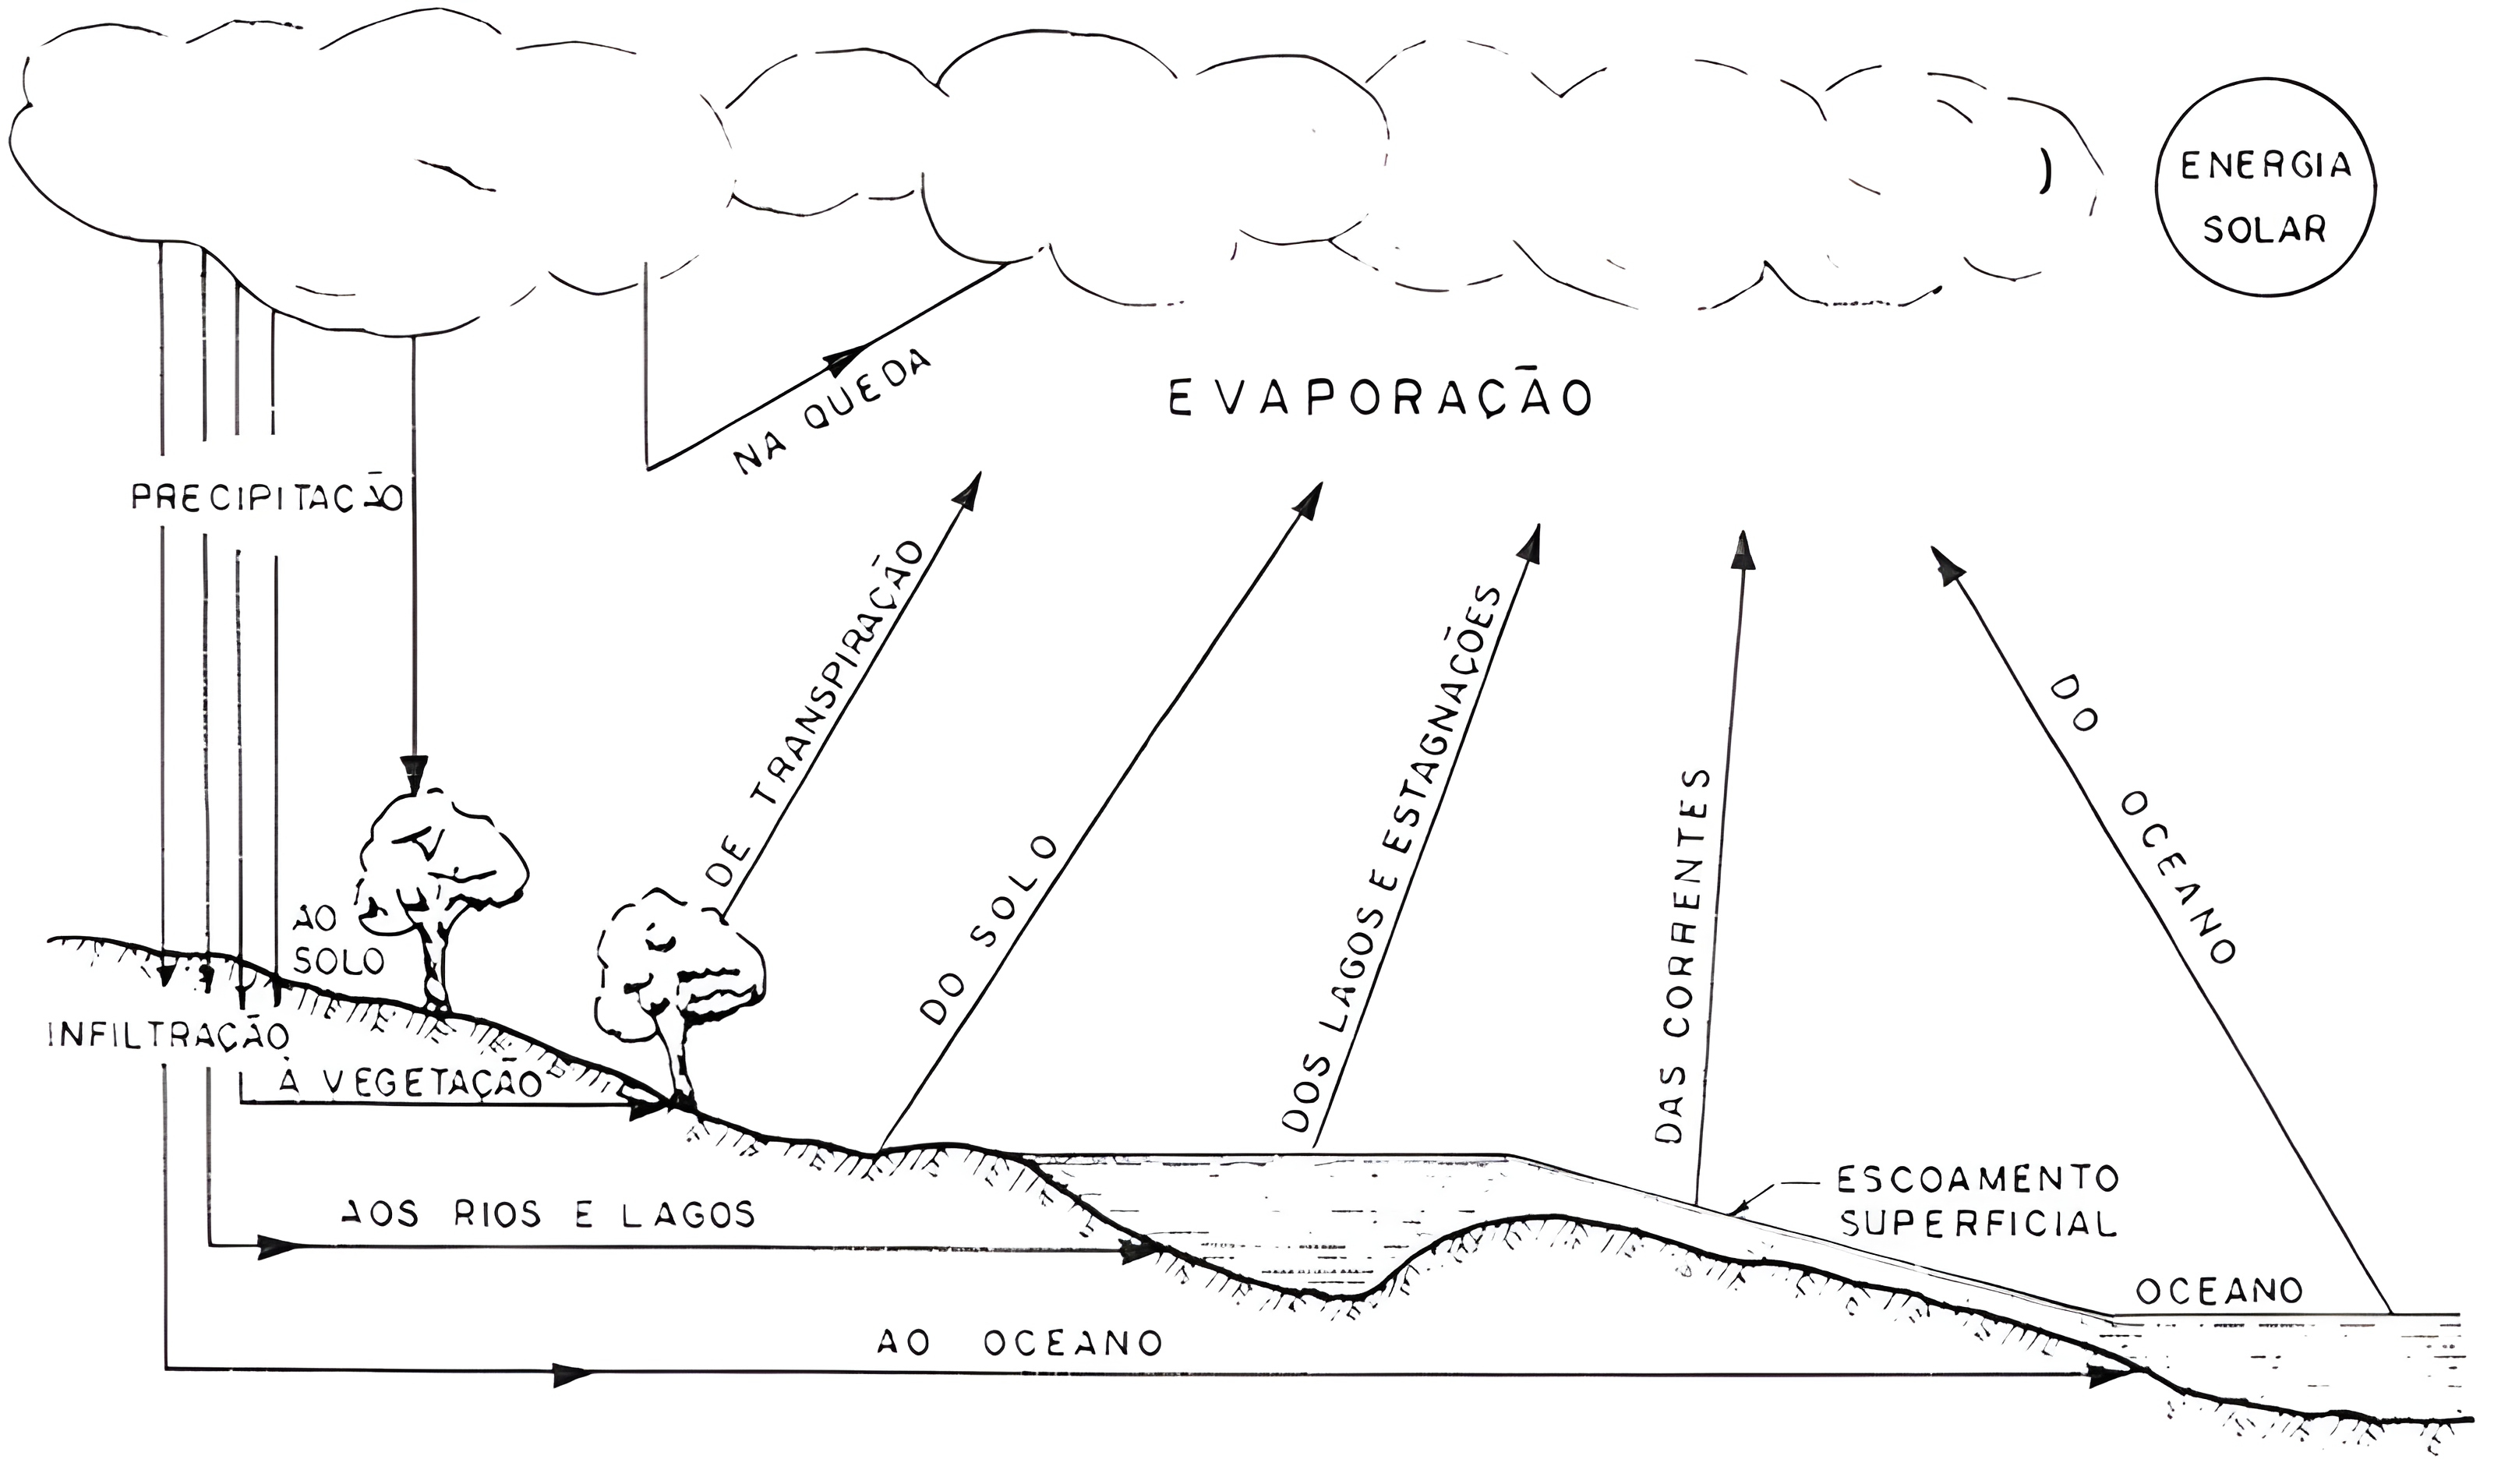
\includegraphics[width=.7625\linewidth]{figuras/ciclo_hidrologico.png}
	\caption*{\textbf{Fonte:} Adaptado de Wilken (1978, p. 2).}
	\label{fig:ciclo_hidrologico.png}
\end{figure}

\section{TIPOS DE PRECIPITAÇÃO}

Existem vários tipos de precipitação, e cada uma delas possui sua própria particularidade. Bertoni e Tucci (2012) classificaram pelo menos sete delas. Eles citam a neve formada por cristais de gelo, a saraiva que consistem em pedras de gelo arredondadas com diâmetros de até cinco milímetros e o granizo que é descrito como pedras de gelo irregulares que possuem diâmetros iguais ou maiores que cinco milímetros.

Também é falado sobre o orvalho e a geada. É dito que o primeiro é a condensação do vapor de água em objetos, formando gotículas em seu entorno, e geralmente acontece devido ao resfriamento noturno. No segundo, o processo é semelhante ao primeiro, porém a água condensada congela, formando cristais de gelo em temperaturas inferiores a 0°. 

Já o chuvisco, é descrito como neblina ou garoa, e é uma precipitação fina de baixa intensidade. Por fim, é falado sobre à chuva, que é o tipo de precipitação que será o foco do presente trabalho, e acontece na forma líquida da água em formato de gotas. 

\section{FORMAÇÃO DAS CHUVAS}

A formação das chuvas se inicia pela água presente na atmosfera em forma de vapor. Todo esse processo acontece através do acúmulo do mesmo em diferentes temperaturas, que vai decaindo ao longo do tempo. Tudo se encaminhará até o ponto em que irá ocorrer a saturação e condensação, iniciando assim a chuva. 

Para Collischonn e Dornelles (2015), as nuvens em geral se formam de maneira associada à movimentação das massas de ar úmido de maneira ascendente. Esse movimento por sua vez, é usado para diferenciar os tipos de chuva, as principais são as orográficas, as convectivas e as frontais também chamadas de ciclônicas.

É possível entender a partir das definições de Bertoni e Tucci (2012) como se dão esses tipos de chuva. Eles explicam as orográficas como de pequena intensidade e grande duração, provindas do deslocamento de ar quente e úmido advindos geralmente do mar indo de encontro às montanhas, que o eleva e resfria, condensando e dando origem a chuva. 

Já as convectivas, eles dizem ser conhecidas por ter uma grande intensidade e pequena duração, e acontecem caracteristicamente em regiões equatoriais, após o ar úmido aquecido e em equilíbrio entorno do solo, elevar-se de forma brusca depois de uma perturbação, gerando por vezes a condensação e a chuva. 

Tratando das chuvas frontais, elas são relatadas como de longas durações e média intensidade, com ventos fortes de circulação ciclônica. Este tipo de chuva advém do impulsionamento à atmosfera gerado pela interação das massas de ar úmido de diferentes temperaturas, ocorrendo então o resfriamento e condensação, podendo assim haver às chuvas. A seguir é possível visualizar o comportamento dos tipos de chuva citadas, na Figura 3.2.\bigskip

\begin{figure}[!ht]
	\centering
	\caption{Tipos de chuva segundo a origem do processo.}
	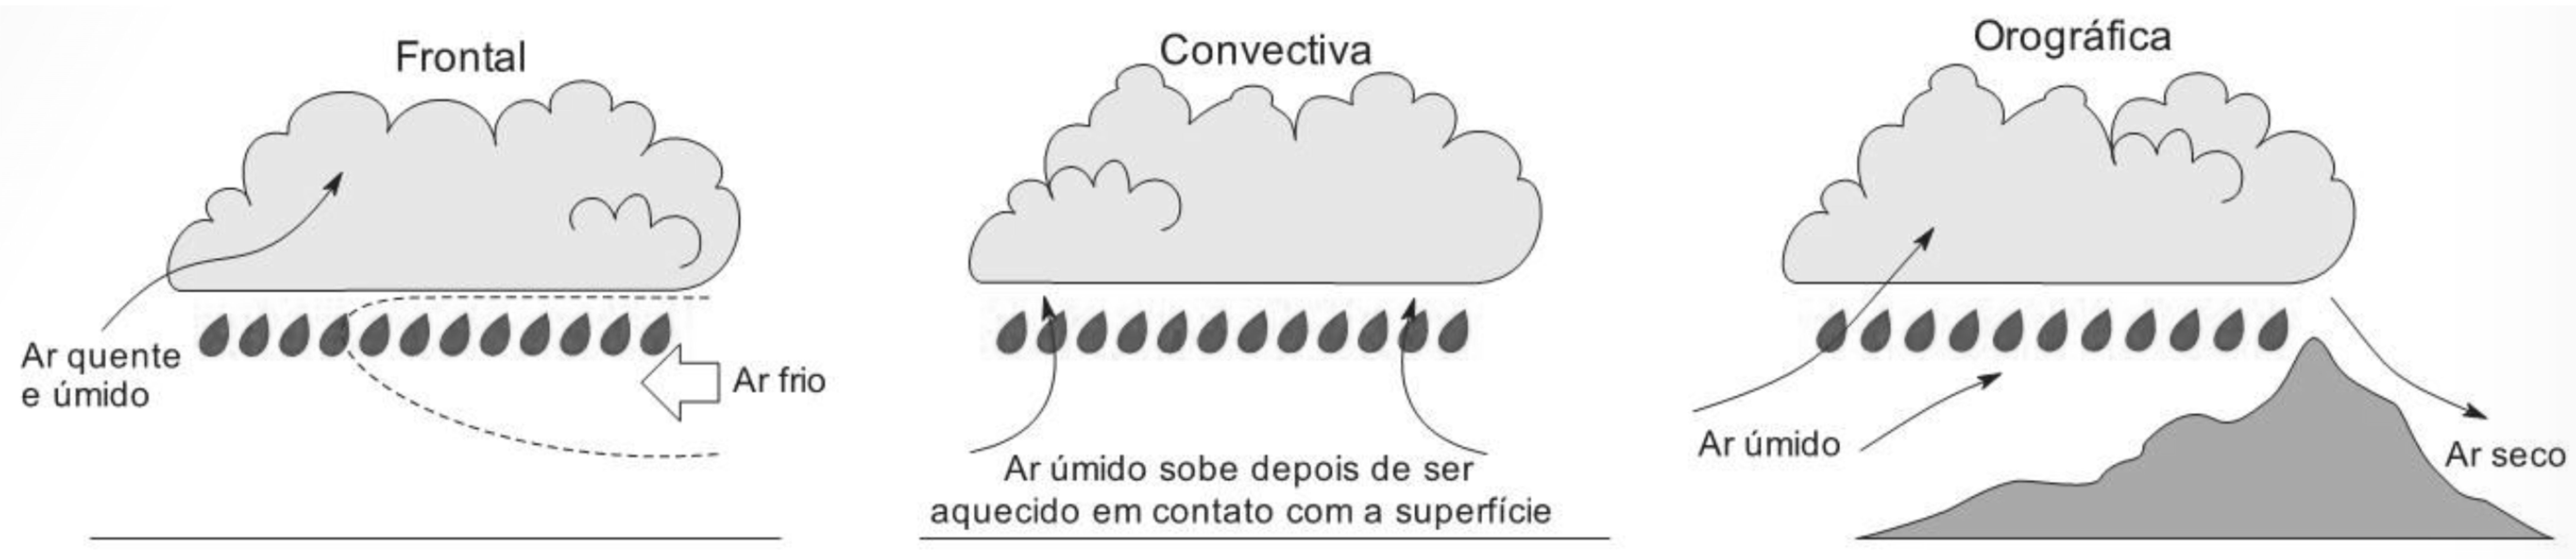
\includegraphics[width=.9\linewidth]{figuras/tipos_de_chuva_segundo_a_origem_do_processo.png}
	\caption*{\textbf{Fonte:} Adaptado de Collischonn e Dornelles (2015, p. 54).}
	\label{fig:tipos_de_chuva_segundo_a_origem_do_processo.png}
\end{figure}

\section{VARIÁVEIS E GRANDEZAS DE CHUVAS}

Independente dos tipos de chuva e a forma como se originam, algumas de suas características se mantém, possibilitando assim que se trace grandezas em comum. Porém, antes de abordar as definições destas feita pela literatura, o entendimento da incerteza em eventos que envolvem o clima, o tempo e a natureza é imprescindível.

A estatística e teoria da probabilidade, incluindo em especial os sistemas estocásticos, são comumente usados para lidar com a imprevisibilidade do comportamento de eventos climáticos como a chuva. A incerteza explicitada nos eventos climáticos faz com que se entenda a ideia de um dos matemáticos que fez grandes contribuições em diversas áreas da estocástica. Gauss (1900) afirma que, mesmo o espaço tendo uma realidade fora da mente, não se pode descrever completamente suas propriedades a priori.

Aplicando esses conceitos aos eventos de precipitação de chuva, é inquestionável que os padrões climáticos geradores da mesma são interconectados, a exemplo da temperatura do ar, da topografia, da umidade, entre outros. Fica claro então, que qualquer variação em qualquer uma dessas variáveis, além dos fatores desconhecidos ou imprevisíveis, podem afetar significativamente às chuvas, dificultando a sua antecipação. 

Assim sendo, a estocástica é usada justamente para lidar com os processos aleatórios gerados por variáveis como as citadas anteriormente, modelando sistemas que se utilizam de probabilidade e estatística, para elaborar previsões através do entendimento do comportamento de sistemas complexos e incertos.

E é a partir desses processos matemáticos que são definidas as grandezas necessárias para estimar e descrever os eventos de precipitações de chuvas, para que assim haja a obtenção de informações que auxiliem nos projetos e dimensionamentos que envolvem águas pluviais. Bertoni e Tucci (2012) descrevem pelo menos quatro grandezas, que por sua vez são usadas para caracterizar as chuvas. 

A altura pluviométrica como sendo uma delas, é relatada como a espessura média da lâmina de uma determinada região, medida habitualmente como milímetro de chuva. Outra delas é a duração, que é resumidamente o período de tempo que ocorre a queda de chuva, representada geralmente em minutos ou horas. 

A intensidade também é definida como uma das grandezas. Observada como a precipitação por unidade de tempo, é a relação da altura pluviométrica pela duração, e se expressa normalmente em milímetros por hora ou milímetros por minuto. Por fim tem-se a frequência de probabilidade e tempo de recorrência, que é a interpretação do número médio de anos em que se é esperado que a precipitação analisada seja igualhada ou superada.

\section{MEDIÇÃO DE CHUVAS}

A medição das chuvas se origina da necessidade de obtenção dos dados, para o desenvolvimento de análises, estudos e previsões. Collischonn e Dornelles (2015) expõem que o instrumento utilizado para medir a chuva é chamado de pluviômetro, sendo os primeiros de medição manual como mostrado na Figura 3.3, ele é definindo como recipientes para coleta da água precipitada com algumas dimensões estabelecidas. Eles são instalados distantes de casas e árvores a uma altura de um metro e meio do solo, para que haja o mínimo de interferência possível na quantidade de água captada.\bigskip

\begin{figure}[!ht]
	\centering
	\caption{Características de pluviômetro manual.}
	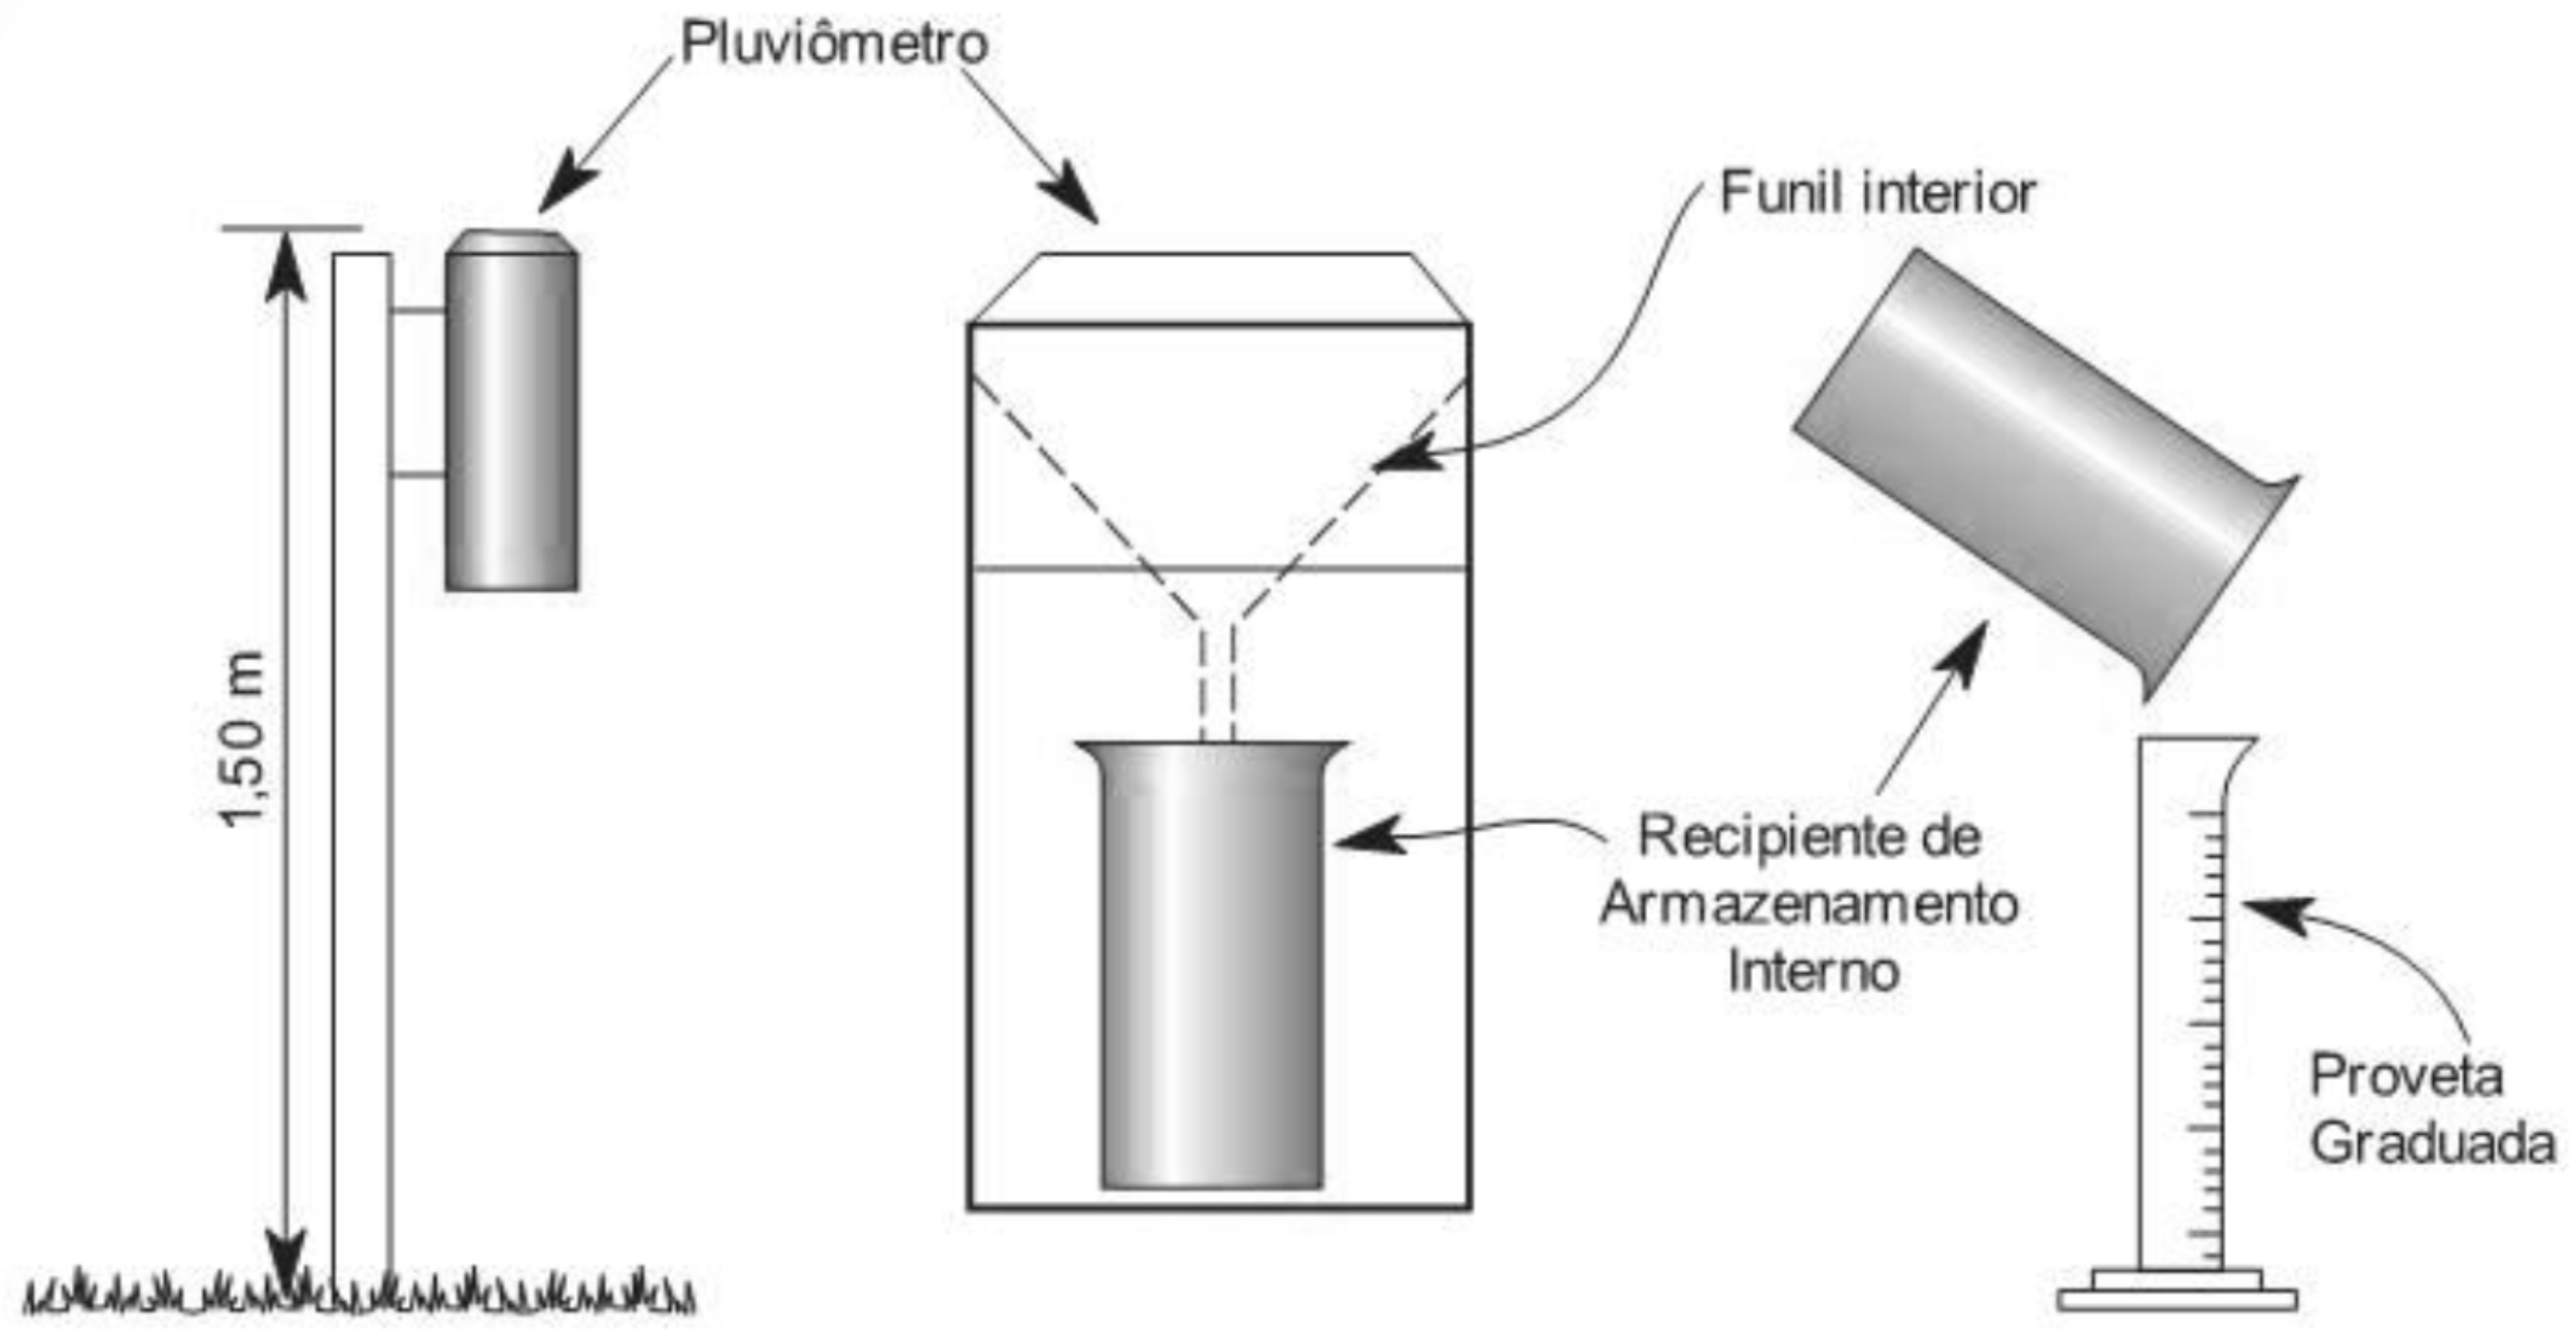
\includegraphics[width=.7625\linewidth]{figuras/caracteristicas_de_um_pluviometro_de_leitura_manual.png}
	\caption*{\textbf{Fonte:} Adaptado de Collischonn e Dornelles (2015, p. 56).}
	\label{fig:caracteristicas_de_um_pluviometro_de_leitura_manual.png}
\end{figure}

Collischonn e Dornelles (2015) também citam os pluviômetros adaptados para medições automáticas, também chamados de pluviógrafos, que de início eram mecânicos e se utilizavam de balança para pesagem e papel para registro. Representados pela Figura 3.4, os atuais são digitais e registram os dados em uma memória. Eles possuem vantagens sobre o pluviômetro de medição manual, visto que consegue analisar de forma mais detalhada a chuva ao longo do dia, além da possibilidade de acoplação a sistemas de transmissão de dados.\bigskip

\begin{figure}[!ht]
	\centering
	\caption{Características de pluviômetro automático de cubas basculantes.}
	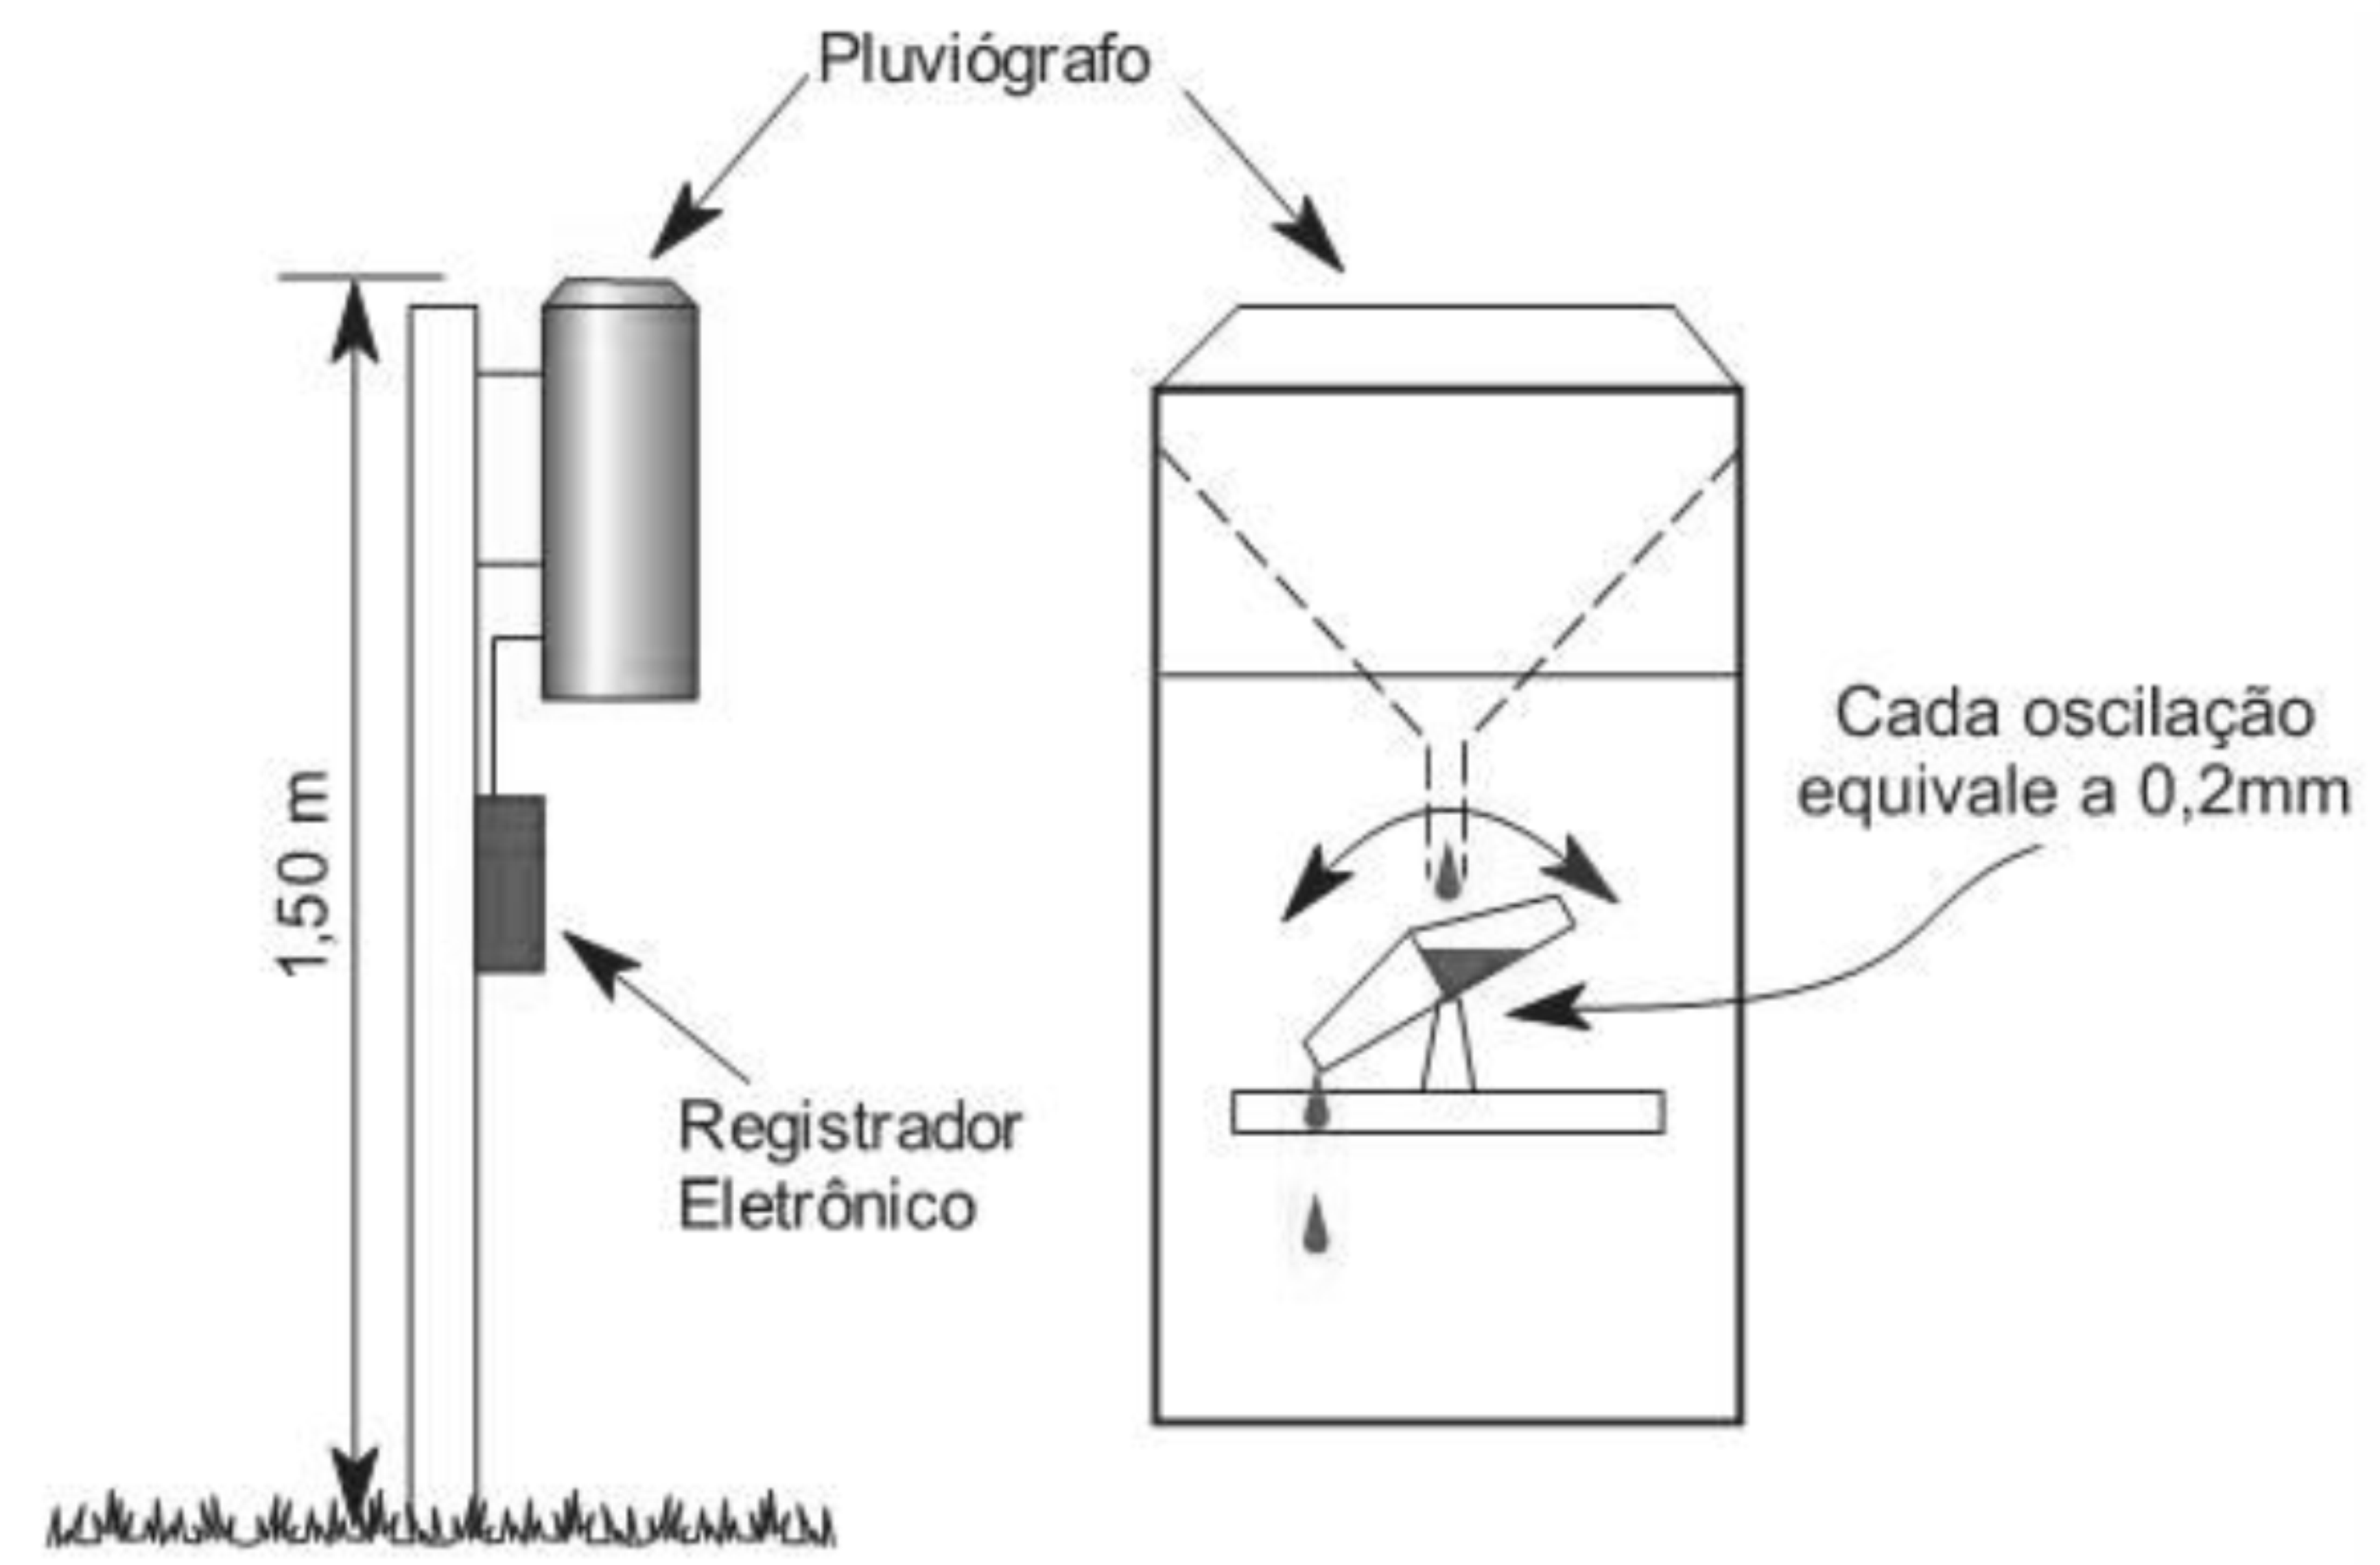
\includegraphics[width=.7625\linewidth]{figuras/caracteristicas_de_um_pluviometro_de_leitura_automatica_baseado_no_mecanismo_de_cubas_basculantes.png}
	\caption*{\textbf{Fonte:} Adaptado de Collischonn e Dornelles (2015, p. 56).}
	\label{fig:caracteristicas_de_um_pluviometro_de_leitura_automatica_baseado_no_mecanismo_de_cubas_basculantes.png}
\end{figure}

\newpage

Existem também outros métodos conhecidos, sendo um deles o de medição de chuva através de radares meteorológicos, que é baseado na emissão de pulsos de radiação eletromagnética refletidos pelas partículas de água de chuva na atmosfera, e medição da intensidade do sinal refletido. Outro método é o da estimativa de precipitação através de imagens retiradas de sensores instalados em satélites.

\section{CHUVAS INTENSAS}

É possível perceber que o estudo acerca do fenômeno que é a chuva é complexo, mas existem caminhos que podem ser seguidos, para que haja a obtenção de bons resultados baseado no que se deseja alcançar. Tendo isso em vista, o presente trabalho trata de um tipo específico de precipitação pluviométrica conhecida como chuva intensa.

Esse tipo de aguaceiro se caracteriza por a queda de uma grande quantidade de água em um curto período de tempo. É perceptível que este tipo de chuva é a causa de problemas diversos como deslizamentos, inundações, destruição em zonas populadas principalmente de baixa infraestrutura, dentre outros desastres naturais.

São notáveis os impactos das chuvas intensas tanto no meio ambiente, como no meio urbano e rural, como observado por Bertoni e Tucci (2012). E restando ao homem adaptar-se a este tipo de evento imposto pela natureza, é possível se utilizar do conhecimento científico e popular, como os apresentados até aqui, para diminuir os impactos, e se aproveitar das benesses desse tipo de evento climático.

\section{EQUAÇÃO DE CHUVAS INTENSAS}

Para explicar e deduzir matematicamente o fenômeno das chuvas intensas, métodos matemáticos que serão explicados mais adiante, são utilizados resultando em curvas que podem ser deduzidas através de uma equação. Ela é chamada por Wilken (1978) de equação intensidade-duração-frequência ou equação de chuvas, também conhecida popularmente como equação de chuvas intensas. Foi desenvolvida para diversos fins, a citar alguns deles, como o dimensionamento de projetos de drenagem de águas pluviais e de barragens, sistemas de irrigação, controles de inundação e planejamento urbano. 

Sobre os cálculos, Wilken (1978) é claro ao afirmar que a equação IDF é gerada a partir das relações entre a intensidade, duração e frequência, que por sinal a nomeiam. Elas são relacionadas através da observação de dados de séries históricas de precipitação em um tempo suficientemente grande para que seja possível aceitar às frequências como probabilidade.  Como resultado, têm-se as curvas mencionadas, de intensidade-duração-frequência para cada frequência, com uma regularidade entre as mesmas que possibilita a tradução uniforme delas através do equacionamento. Existem equações que podem ser usadas para explicar as curvas matematicamente, porém apenas uma será tratada neste trabalho que é a apresentada a seguir, descrita por Bertoni e Tucci (2012) como genérica e boa representante das frequências citadas.\bigskip

\newpage

\begin{equation}
I = \frac{a * Tr^b}{(t + c)^d}
\end{equation}
\newline
onde:
\newline
\textit{I} é a intensidade da chuva, (mm/h);
\newline
\textit{Tr} é o tempo de retorno, (ano);
\newline
\textit{t} é a duração, (min);
\newline
\textit{a, b, c, d}  são os parâmetros da equação da intensidade das chuvas, (adimensional).\bigskip

Sabendo disso, é necessário entender os processos matemáticos que levam aos resultados que se desejam, que são os parâmetros da equação da intensidade das chuvas. Baseado nos resumos esquemáticos dos estudos de Pinto (2013) e de Neto (2020), foi elaborado para o presente trabalho um fluxograma visualizado através da Figura 3.5, que define os passos a se seguir para determinar os parâmetros da equação IDF.\bigskip

\begin{figure}[!ht]
	\centering
	\caption{Fluxograma de equação das chuvas intensas.}
	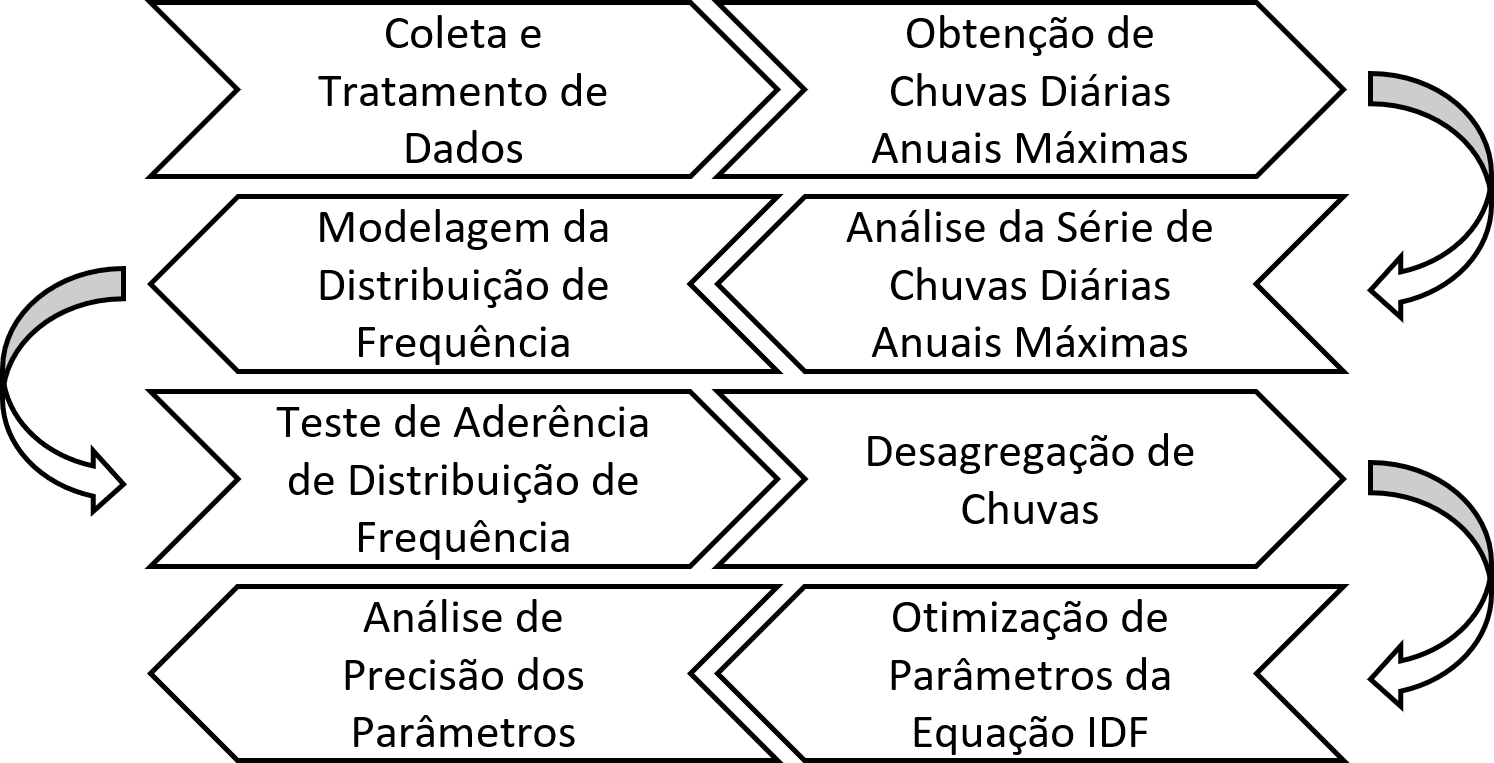
\includegraphics[width=.7625\linewidth]{figuras/fluxograma_de_equacao_idf.png}
	\caption*{\textbf{Fonte:} De autoria própria (2023).}
	\label{fig:fluxograma_de_equacao_idf.png}
\end{figure}

\subsection{O tratamento de dados}

A partir da coleta de dados já explicada, é preciso pensar sobre as falhas presente neles. É comum a falta de informações de precipitação em alguns dias durante o ano. Se tratando de dados de chuvas, devido a incerteza presente nesses eventos temporais, são notórias as dificuldades que se encontra para os preenchimentos de suas falhas. Para um melhor entendimento, é possível usar de exemplo regiões onde a variação do tempo é brusca, e a maioria dos dias do ano simplesmente não chove, além das chuvas esporádicas entre os dias de estiagem, tornando o preenchimento das falhas extremamente problemático. 

Para que se faça uma boa análise de dados falhos, é importante estabelecer um limiar de falhas que caso ultrapassado, desconsidera-se a série analisada. É possível estabelecer esse limite de forma empírica, como no caso de trabalhos como o de Santos (2017) e Beskow \textit{et al.} (2013), e de forma estatística, como no estudo de Kim e Ryu (2015).

Caso o limiar não seja ultrapassado, é possível utilizar métodos de preenchimento de dados. Bertoni e Tucci (2012) descrevem os de ponderação regional, regressão linear simples e múltipla, e até mesmo a ponderação regional com base em regressões lineares. Os autores destacam que essas formas de preenchimento de falhas são principalmente usadas em séries mensais e anuais. A interpolação também é uma maneira viável de preencher falhas, e será explicada em um tópico mais adiante.

Uma forma mais simples de lidar com dados ausentes é a explicada por Allison (2001), chamada de \textit{complete case analysis}, que apenas exclui os dados ausentes. O autor a descreve como de fácil implementação, porém destaca que deve ser usada com cuidado visto que a depender das falhas, ela pode excluir uma grande parcela da amostra original. Cabe ao calculista analisar e decidir qual método melhor se encaixa nas especificação de sua base de dados.

\subsection{As chuvas diárias anuais máximas}

Em posse dos devidos dados, faz-se importante a análise da quantidade de anos que se tem informações de precipitação, e a interpretação de diferentes autores sobre qual seria o mínimo tempo necessário de medição de dados de chuva diária para que sejam desenvolvidas as frequências probabilísticas. Isto porque bons dados iniciais influenciam diretamente na precisão das previsões de intensidade feitas com a equação IDF.

O Instituto Nacional de Pesquisas Espaciais (INPE) recomenda que para o comportamento estatístico das variáveis de tempo como temperatura, chuva e vento, possua-se dados de um período de pelo menos 30 anos. Porém, devido a escassez de informações para um tempo tão longo, alguns autores admitem menores períodos mínimos. É possível comprovar essa afirmação através de estudos como o de Pfafstetter (1957), que elaborou equações com dados de 98 postos meteorológicos ao longo de todo o Brasil, possuindo elas séries históricas com uma média de aproximadamente 22 anos. É visível também no trabalho de Martinez e Magni (1999), convênio do Departamento de Águas e Energia Elétrica e da Escola Politécnica da Universidade de São Paulo, a apresentação de períodos de anos menores que o recomendado pelo INPE, com uma média de 27 anos para 30 cidades do estado brasileiro de São Paulo.

Compreendendo essa questão, organiza-se os dados que serão usados no cálculo da equação das chuvas intensas e se seleciona a maior chuva diária de cada ano do conjunto de dados. Em posse da série histórica de chuva diária anual máxima, aplica-se o teste de Mann-Kendall (MK) proposto por Helsel \textit{et al.} (2020), para busca por tendências em dados hidrológicos, que indica entre outros questões as mudanças climáticas, que por sua vez podem afetar previsões estatísticas.

\subsection{A modelagem probabilística}

Não havendo tendência na série de precipitações máximas diárias anuais, segue-se para modelagem probabilística dos dados de precipitação máxima diária anual, que é feita através de distribuições de probabilidade. Estas são usadas para análise de frequência, e estimam as precipitações para diferentes tempos de retorno. Dito isso, nota-se a existência de variadas distribuições, que se ajustam de maneiras diferentes a depender dos dados, resultando em precisões diversas. 

A escolha da distribuição probabilística para a modelagem será sempre a que, quando comparada com outras que apresentam bons ajustes para dados hidrológicos, terá a melhor precisão. Sabendo disso, é possível citar às distribuições de probabilidade Exponencial, Gama, de Gumbel, e Log-Normal que possuem dois parâmetros. Quando se trata de possuir três parâmetros, têm-se as Generalizada de Pareto, Logística Generalizada, Normal Generalizada, de Pearson tipo III, e de Weibull. Com quatro parâmetros, menciona-se a de Kappa 4.

Neghettini e Pinto (2007) tratando de hidrologia estatística, analisam todas as distribuições probabilísticas citadas, com exceção de Kappa 4. Lanna (2012) em sua abordagem de modelos probabilísticos cita como boas para aplicação na hidrologia as distribuições Exponencial, Gama, de Gumbel, Log-Normal, Normal e de Weibull. 

Já Pinto (2013) em seu trabalho de elaboração da metodologia de cálculo das equações IDF para o Atlas Pluviométrico do Brasil, utiliza das distribuições de probabilidade Exponencial, Gama, de Gumbel, Generalizada de Pareto, e Generalizada Logística. Como única com quatro parâmetros, a distribuição de probabilidade de Kappa 4 se faz necessária para comparação com outras funções de menor quantidade de parâmetros, sendo descrita por Hosking e Wallis (1997) como ótima para este fim, aumentando a precisão dos modelos estatísticos.

Os parâmetros das distribuições citadas, necessitam de um método estimativo que facilite o seu cálculo, e ao mesmo tempo gere precisão. Entre os métodos citados por Neghettini e Pinto (2007), têm-se o da máxima verossimilhança (MVS), sendo ele destacado como o de maior eficiência por produzir os estimadores de menor variância.

\subsection{As funções de aderência de distribuições probabilísticas}

A escolha de uma distribuição probabilística, também está ligada a aderência que ela têm com os dados utilizados. Para conferir se os dados observados estão realmente bons, precisa-se de um método estatístico que verifique se eles são provenientes de uma distribuição determinada. 

Dentre os principais testes de aderência citados por Neghettini e Pinto (2007) empregados em hidrologia estatística, é possível citar o de Kolmogorov-Smirnov (KS) e o de Anderson-Darling (AD). Como explicado pelos autores, eles comparam as funções de distribuição acumulada empíricas das teóricas.

Neste sentido, há um calculo estatístico de teste que mede a distância entre elas, descrita como a diferença máxima entre as duas distribuições. No caso dela ser maior que um valor crítico, encontrado a partir da significância arbitrada, então a hipótese nula é rejeitada e conclui-se que as amostras são extraídas de distribuições de probabilidade diferentes.

\subsection{A desagregação de dados pluviométricos}

Após definir uma distribuição de probabilidade que se adéque aos dados observados, é necessário estabelecer uma relação entre as precipitações das chuvas e suas durações. Como é dito por Back e Wildner (2021), inicialmente ela era estabelecida a partir da observação das chuvas de curta duração através de pluviógrafos.

Porém como explicado anteriormente, existe uma enorme dificuldade na obtenção de longas séries de dados devido a escassez dessas informações no vasto território brasileiro. E essa afirmação é endossada em diversos trabalhos, a citar o de Cecílio e Pruski (2003), que visa contornar esse problema através da interpolação dos parâmetros da equação IDF.

Entretanto, uma maneira eficaz de encarar a carência de dados é através da desagregação das chuvas. Explicada por Bertoni e Tucci (2012) por meio do método da relação entre durações, nele são aplicados os coeficientes de correção elaborados para desagregar chuvas máximas anuais de um dia em precipitações pluviométricas de menores durações.

Os coeficientes mais utilizados em estudos e projetos que recorrem à desagregação de chuvas no Brasil, são os desenvolvidos pela DAEE/CETESB (1980), que podem ser observados na Tabela 3.1, elaborados para abranger todo o território nacional.\bigskip

\begin{table}[ht]
\centering
\caption{Relação entre chuvas de diferentes durações.}
\begin{tabular}{
>{\columncolor[HTML]{FFFFFF}}c
>{\columncolor[HTML]{FFFFFF}}c }
\hline
\rowcolor[HTML]{FFFFFF} 
\begin{tabular}[c]{@{}c@{}}Relação entre Alturas \\ Pluviométricas\end{tabular} & \begin{tabular}[c]{@{}c@{}}Coeficientes de \\ Desagregação\end{tabular} \\ \hline
\rowcolor[HTML]{FFFFFF} 
05 min / 30 min & 0.34 \\
\rowcolor[HTML]{FFFFFF} 
10 min / 30 min & 0.54 \\
\rowcolor[HTML]{FFFFFF} 
15 min / 30 min & 0.70 \\
\rowcolor[HTML]{FFFFFF} 
20 min / 30 min & 0.81 \\
\rowcolor[HTML]{FFFFFF} 
25 min / 30 min & 0.91 \\
\rowcolor[HTML]{FFFFFF} 
30 min / 01 h & 0.74 \\
\rowcolor[HTML]{FFFFFF} 
01 h / 24 h & 0.42 \\
\rowcolor[HTML]{FFFFFF} 
06 h / 24 h & 0.72 \\
\rowcolor[HTML]{FFFFFF} 
08 h / 24 h & 0.78 \\
\rowcolor[HTML]{FFFFFF} 
10 h / 24 h & 0.82 \\
12 h / 24 h & 0.85 \\ \hline
\end{tabular}
\caption*{\textbf{Fonte:} DAEE/CETESB (1980, p. 22).}
\end{table}

Bertoni e Tucci (2012) avaliam que o coeficiente da relação de 1 dia para 24 horas pode ser menor em regiões onde chuvas convectivas são predominantes. O valor fixado neste estudo será de 1.14, utilizado na cidade de São Paulo.

\newpage

No trabalho da DAEE/CETESB (1980), também é possível ver diversos coeficientes de desagregação de outras fontes, a exemplo dos adotados pelo \textit{United State Weather Bureau} conhecida atualmente por \textit{National Weather Service} (NWS). Logo, fica claro é possível se utilizar de coeficientes de desagregação de outras fontes, ou até mesmo elaborados pelo próprio calculista. Com base na Tabela 3.1, Silveira (2000) desenvolveu a equação (3.2) com o menor erro possível através de regressões lineares e ajustes bi-logarítmicos, permitindo uma maior flexibilidade nos cálculos para durações iguais ou maiores a 5 minutos e menores que 24 horas.\bigskip

\begin{equation}
C = e^{1.5 * \ln{\left(\frac{ln{\left(t\right)}}{7.3}\right)}}
\end{equation}
\newline
onde:
\newline
\textit{C} é o coeficiente de desagregação, (adimensional);
\newline
\textit{e} é a constante de Euler, (adimensional);
\newline
\textit{t} é a duração qual se quer extrair o coeficiente, (min).\bigskip

\subsection{Os métodos de otimização para ajuste de parâmetros de funções}

As intensidades nascem da relação entre as precipitações desagregadas em chuvas de menores durações, e as durações que definiram os coeficientes. Obtidas às intensidades, Wilken (1978) descreve a análise da frequência que estabelece uma relação analítica já explicada entre a intensidade, a duração e a frequência. Traça-se então, curvas dos pontos das várias frequências com as intensidades nas ordenadas, e as durações nas abscissas, vistas na Figura 3.6.\bigskip

\begin{figure}[!ht]
	\centering
	\caption{Curvas da relação entre intensidade e duração.}
	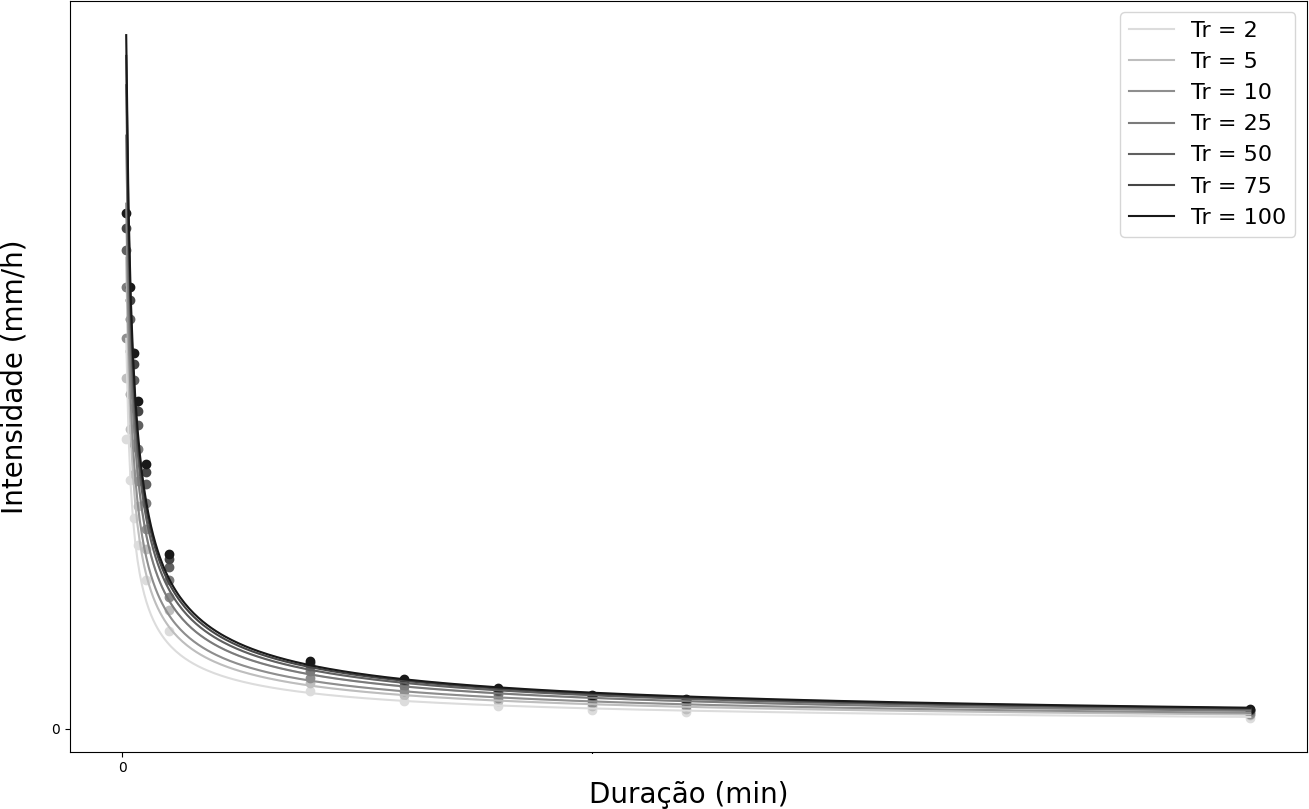
\includegraphics[width=.7325\linewidth]{figuras/curvas_idf_de_intensidade_e_duracao.png}
	\caption*{\textbf{Fonte:} De autoria própria (2023).}
	\label{fig:curvas_idf_de_intensidade_e_duracao.png}
\end{figure}

\newpage

Reiterando que os tempos de retorno definidos são as frequências citadas inicialmente, onde são geradas curvas para cada uma delas com a mesma forma geral citada anteriormente, visto que elas possuem séries de intensidades diferentes.

Para a obtenção dos parâmetros da fórmula (3.1), que representa todas as curvas numericamente, se fazem necessários métodos de otimização matemática, que podem ser desenvolvidos através de cálculos manuais, ou de algoritmos projetados para encontrar valores mínimos ou máximos a partir de iteração e métodos numéricos avançados.

O mais simples dentre os que serão citados é justamente um que se utiliza apenas do calculo manual, em prol de extrair as funções das curvas. Denominado de método dos mínimos quadrados (MMQ), foi descoberto e justificado pelo matemático Carl F. Gauss como descrito por Boyer (1968). Nele serão utilizadas a função com ajustes de potência, para gráficos em que a disposição dos pontos tendem a formar curvas, e a com ajustes lineares para gráficos que seus pontos tendem a estar dispostos em forma de reta.

Já os de otimização que se utilizam de algoritmos, necessitam de implementação em linguagens de programação para seu pleno funcionamento, promovendo robustez em suas buscas, além de precisão a depender de seus números para partida, intervalos de busca referentes aos parâmetros a se ajustar, além da quantidade de interações. Inicialmente esses métodos eram implementados em linguagens de programação de baixo nível, que desenvolviam as execuções dos mesmos promovendo alto desempenho. 

Com o avanço da tecnologia, foi possível desenvolver otimizações de funções em linguagens de programação de alto nível. O presente trabalho dá enfoque ao Python, que através de bibliotecas como o NumPy e SciPy, pode usar esses métodos de forma ágil ao utilizar a compilação de suas rotinas mais críticas nas linguagens de programação de baixo nível, em especial C, C++ e Fortran. Vale ressaltar que as bibliotecas citadas são desenvolvidas em código aberto, promovendo acessibilidade e avanço científico. 

Partindo para métodos de otimização global que visam o ajuste de multiplos parâmetros de uma função disponibilizados pelo SciPy e adequados à dados com séries hidrológicas, é possível citar os determinísticos e os estocásticos. Para o primeiro, tem-se \textit{Constrained Optimization By Linear Approximations} (COBYLA), \textit{Conjugate Gradient} (CG), Broyden-Fletcher-Goldfarb-Shanno (L-BFGS-B), Levenberg-Marquardt (LM), Nelder-Mead (NM), Powell e \textit{Truncated} Newton (TNC). Já em relação ao segundo, cita-se \textit{Dual-Annealing} (DA) e \textit{Differential Evolution} (DE).

A escolha de qual utilizar para encontrar os melhores parâmetros, que representam as curvas de frequência em uma equação IDF, dependerá unicamente da precisão que desempenharão de acordo com os dados e necessidades informadas pelo calculista. A melhor resposta nascerá da tentativa e erro, que é desenvolvida pela máquina de processamento ao relacionar a melhor modelagem probabilística junto do melhor método de otimização.

\newpage

O desempenho dos resultados representado pelo grau de sua precisão, que informará qual equação IDF melhor se ajustou aos dados informados após as sucessivas tentativas explicadas anteriormente, será determinado a partir do coeficiente de Nash e Stucliff (NS) (1970), que detalharam seu uso para dados hidrológicos. Ele varia de infinito negativo até a maior precisão possível representada pelo número um. Já para viés de aferição em conjunto com NS, é possível usar a Raiz do Erro Quadrático Médio (RMSE), onde o seu resultado representará na unidade de medida da intensidade, o seu erro para mais ou para menos.

\subsection{O cálculo manual da equação de chuva intensas}

É bem verdade que a otimização usada no ajuste dos parâmetros da equação das chuvas intensas, torna o todo o cálculo envolto a ela menos tátil, visto que o uso de algoritmos computacionais se torna essencial para resultados satisfatórios. Porém é importante dizer que os passos para chegar a equação se mantém, que é o tratamento de dados, seguido da modelagem probabilística, para que assim haja a desagregação e geração das curvas de intensidade, duração e frequência, e a partir delas se descubra os parâmetros e a equação IDF.

Tendo isso em mente, se faz importante entender esses passos de uma maneira menos abstrata, através de equações e do cálculo manual, empregando as fórmulas matemáticas para a obtenção de um resultado. Obviamente o nível de precisão não é o mesmo que o de um computador que itera múltiplas vezes diferentes distribuições de frequência e otimizações, em busca da solução ideal. Porém é de se pensar que a observação de cálculos palpáveis torna bem mais digerível o entendimento dos processos que os próprios algoritmos levam em busca de ajustes para a equação que melhor representem os dados observados.

Pensando nisso, o presente tópico visa abordar as partes mais sensíveis do cálculo da equação das chuvas intensas, que é a modelagem probabilística, a desagregação e a elaboração das curvas IDF, encontrando a partir delas a equação das chuvas intensas. Não será abordada a parte de tratamento de dados inicial, focando apenas no cálculo da equação a partir de precipitações máximas diárias anuais já determinadas para uso. Será possível observar um exemplo seguindo os passos apresentados, no apêndice do trabalho. \bigskip

\subsubsection{As distribuição de frequências}\bigskip

Iniciando a modelagem probabilística, para o cálculo da distribuição de frequências optou-se pelo uso de Gumbel, por ser um método de cálculo relativamente simples, com apenas dois parâmetros. O cálculo se inicia com a média das precipitações diárias anuais máximas (3.3), obtidas a partir dos dados coletados.\bigskip

\newpage

% Média das Precipitações Máximas
\begin{equation}
\bar{X} = \frac{\sum(Xi)}{n}
\end{equation}
\newline
onde:
\newline
$\bar{X}$ é a média das precipitações diárias anuais máximas, (mm);
\newline
$X_i$ é a precipitação diária anual máxima, (mm);
\newline
\textit{n} é o número total de anos precipitados, (adimensional).\bigskip
 
Após descobrir a média das precipitações diárias anuais máximas (3.3), é possível fazer o calculo do desvio padrão (3.4).\bigskip

% Desvio Padrão
\begin{equation}
\delta = \sqrt{\frac{\sum(Xi - \bar{X})^2}{n - 1}}
\end{equation}
\newline
onde:
\newline
$\delta$ é o desvio padrão, (adimensional);
\newline
$X_i$ é a precipitação diária anual máxima, (mm);
\newline
$\bar{X}$ é a média das precipitações diárias anuais máximas, (mm);
\newline
\textit{n} é o número total de anos precipitados, (adimensional).\bigskip

Em posse do desvio padrão (3.4), consegue-se encontrar o parâmetro de escala da distribuição de Gumbel (3.5).\bigskip

% Parâmetro de escala da distrubuição
\begin{equation}
\beta_{1} = \sqrt{\frac{6}{\pi}} * \delta
\end{equation}
\newline
onde:
\newline
$\beta_{1}$ é o parâmetro de escala da distribuição, (adimensional);
\newline
$\pi$ é a constante pi, (adimensional);
\newline
$\delta$ é o desvio padrão, (adimensional).\bigskip

Com a obtenção do parâmetro de escala de distribuição (3.5), junto da média das precipitações diárias anuais máximas de (3.3), tem-se agora o necessário para encontrar a moda de Gumbel (3.6).\bigskip

% Moda de Gumbel
\begin{equation}
\mu = \bar{X} - \gamma * \beta_{1}
\end{equation}
\newline
\newline
onde:
\newline
$\mu$ é a moda de Gumbel, (mm);
\newline
$\bar{X}$ é a média das precipitações máximas, (mm);
\newline
$\gamma$ é a constante de Euler-Mascheroni, (adimensional);
\newline
$\beta_{1}$ é o parâmetro de escala da distribuição de Gumbel, (adimensional).\bigskip

O próximo passo é encontrar da mediana de Gumbel adaptada ao cálculo das precipitações máximas (3.7). Para acha-la, é necessário arbitrar tempos de retorno. Comumente, estes períodos são decididos a partir da análise da região e dos dados utilizados inicialmente.\bigskip

% Mediana de Gumbel (Precipitação de 24 Horas sem Majoração)
\begin{equation}
Xt = \mu - \beta_{1} * \ln{\left(\ln{\left(\frac{Tr}{Tr - 1}\right)}\right)}
\end{equation}
\newline
onde:
\newline
\textit{Xt} é a mediana de Gumbel, (mm);
\newline
$\mu$ é a moda de Gumbel, em (mm);
\newline
$\beta_{1}$ é o parâmetro de escala da distribuição de Gumbel, (adimensional);
\newline
\textit{Tr} é o tempo de retorno, (ano).\bigskip

Por fim tem-se a função cumulativa de Gumbel (3.8), que dirá qual a probabilidade de ocorrer uma chuva de precipitação $Xt$ (3.7) nos determinados tempos de retorno arbitrados.\bigskip

% Função Cumulativa de Chow-Gumbel
\begin{equation}
F(Xt) = e^{- e^{- \frac{Xt - \mu}{\beta_{1}}}}
\end{equation}
\newline
onde:
\newline
\textit{F(Xt)} é a função cumulativa de Gumbel, (porcentagem);
\newline
\textit{e} é a constante de Euler, (adimensional);
\newline
\textit{Xt} é a mediana de Gumbel, (mm);
\newline
$\mu$ é a moda de Gumbel, (mm);
\newline
$\beta_{1}$ é o parâmetro de escala da distribuição, (adimensional).\bigskip

\subsubsection{O Teste de aderência}\bigskip

O teste de aderência utilizado será o mais generalista dentre os citados, que é o de Kolmogorov-Smirnov. Para iniciar o cálculo, descobre-se os parâmetros de posição (3.9) e de escala (3.10) do teste de aderência. Nas fórmulas serão usados a média das precipitações diárias anuais máximas (3.3) e o desvio padrão (3.4).\bigskip

% Parâmetro de posição de KS
\begin{equation}
\beta_{2} = \bar{X} - 0.45 * \delta
\end{equation}
\newline
onde:
\newline
$\beta_{2}$ é o parâmetro de posição de Kolmogorov-Smirnov, (adimensional);
\newline
$\bar{X}$ é a média das precipitações máximas, (mm);
\newline
$\delta$ é o desvio padrão, (adimensional).\bigskip

% Parâmetro de escala de KS
\begin{equation}
\alpha = \frac{\delta}{1.283}
\end{equation}
\newline
onde:
\newline
$\alpha$ é o parâmetro de escala de Kolmogorov-Smirnov, (adimensional);
\newline
$\delta$ é o desvio padrão, (adimensional).\bigskip

Calculados os parâmetros, ordena-se as precipitações de forma decrescente, e após isso, numera-se cada uma de forma crescente, para que assim se calcule a frequência das precipitações diárias anuais máximas dos anos da distribuição (3.11).\bigskip

% Frequência
\begin{equation}
Fr = \frac{i}{n}
\end{equation}
\newline
onde:
\newline
\textit{Fr} é a frequência da distribuição analisada, (porcentagem);
\newline
\textit{i} é a posição do ano precipitado, (mm);
\newline
\textit{n} é o número total de anos precipitados, (adimensional).\bigskip

Com a frequência, encontra-se a frequência não excedida das precipitações diárias anuais máximas (3.12), utilizando o parâmetro de posição (3.9), e o parâmetro de escala (3.10).\bigskip

% Frequência não excedida de Chow-Gumbel
\begin{equation}
Fr_{n\_Exced} = e^{- e^{- \frac{Xi - \beta_2}{\alpha}}}
\end{equation}
\newline
onde:
\newline
$Fr_{n\_Exced}$ é a frequência não excedida da distribuição analisada, (porcentagem);
\newline
\textit{e} é a constante de Euler, (adimensional);
\newline
\textit{Xi} é a precipitação anual máxima, (mm);
\newline
$\beta_2$ é o parâmetro de posição, (adimensional);
\newline
$\alpha$ é o parâmetro de escala, (adimensional).\bigskip

Já para encontrar a frequência excedida (3.13), basta fazer a diferença de um pela frequência não excedida (3.12).

% Frequência excedida de Chow-Gumbel
\begin{equation}
Fr_{Exced} = 1 - Fr_{n\_Exced}
\end{equation}
\newline
onde:
\newline
$Fr_{Exced}$ é a frequência excedida da distribuição analisada, (porcentagem);
\newline
$Fr_{n\_Exced}$ é a frequência não excedida da distribuição analisada, (porcentagem).\bigskip

O próximo passo é encontrar a diferença (3.14), que é descoberta após fazer o módulo da subtração da frequência (3.11) pela frequência excedida (3.13).\bigskip

% Diferença
\begin{equation}
Dn = Fr - Fr_{Exced}
\end{equation}
\newline
onde:
\newline
\textit{Dn} é a diferença, (porcentagem);
\newline
\textit{Fr} é a frequência, (porcentagem);
\newline
$Fr_{Exced}$ é a frequência excedida de Gumbel, (porcentagem).\bigskip

Para finalizar os cálculos do método de KS, busca-se o valor crítico da estatística (3.15) com base na fórmula de sua determinada significância. Sabendo que quanto menor for a porcentagem desse valor, mais precisa será a aderência, têm-se fórmulas para os níveis de um e cinco por cento de significância. Será escolhida aquela que após ponderação, melhor se ajusta à realidade dos dados utilizados.\bigskip

% Valor Crítico de 1%
\begin{equation}
Crit_1 = \frac{1.6276}{\sqrt{n}}
\end{equation}
\newline
onde:
\newline
$Crit_1$ é o valor crítico da estatística de 1\%, (porcentagem);
\newline
\textit{n} é o número total de anos precipitados, (adimensional).\bigskip

% Valor Crítico de 5%
\begin{equation}
Crit_5 = \frac{1.3581}{\sqrt{n}}
\end{equation}
\newline
onde:
\newline
$Crit_5$ é o valor crítico da estatística de 5\%, (porcentagem);
\newline
\textit{n} é o número total de anos precipitados, (adimensional).\bigskip

Após calcular todas as diferenças (3.14) basta comparar a maior diferença com o valor crítico arbitrado (3.15) ou (3.16). Caso a maior diferença for menor que o valor crítico estatístico, a aderência é boa, caso contrário a hipótese nula deve ser rejeitada, como se segue na sentença (3.17).\bigskip

% Hipótese de KS
\begin{equation}
\begin{cases}
Dn_{max}<Crit,&\mbox{\textit{Boa }}\mbox{\textit{Aderência!}} \\
Dn_{max}>Crit,&\mbox{\textit{Hipótese }}\mbox{\textit{Rejeitada!}}
\end{cases}
\end{equation}
\newline
onde:
\newline
$Dn_{max}$ é a diferença máxima, (porcentagem);
\newline
\textit{Crit} é o valor crítico da estatística, (porcentagem).\bigskip

\subsubsection{A Desagregação a partir da relação entre durações}\bigskip

Obtendo uma boa aderência verificada pelo método de KS, segue-se para a desagregação dos dados obtidos de Gumbel, utilizando a equação (3.2) para as durações arbitradas no cálculo.

Após determinar os coeficientes, basta fazer o produto deles pelas precipitações de diferentes períodos de retorno obtidas na fórmula (3.7), resultando nas chuvas desagregadas em durações menores para cada tempo de retorno escolhido (3.18).\bigskip

\begin{equation}
Pr = Xt * C
\end{equation}
\newline
onde:
\newline
\textit{Pr} é a precipitação desagregada, (mm);
\newline
\textit{Xt} é a mediana de Gumbel, (mm);
\newline
\textit{C} é o coeficiente de desagregação, (adimensional).\bigskip

Com as precipitações desagregadas para seus determinados frequências, que neste caso são os períodos de retorno, é possível definir intensidades da chuva precipitada (3.19), a partir do quociente entre precipitações desagregadas e as durações.\bigskip

\begin{equation}
I = \frac{Pr}{t}
\end{equation}
\newline
onde:
\newline
\textit{I} é a intensidade para uma determinada duração, (mm/h);
\newline
\textit{Pr} é a precipitação desagregada, (mm);
\newline
\textit{t} é a duração da determinada precipitação, (h).\bigskip

Após ter as intensidades encontradas, é possível gerar as curvas de frequência já mencionadas, relacionando-as com as durações arbitradas. A Figura 3.2 explicita o que foi falado, sendo cada curva representada por uma cor, um tempo de retorno diferente, e cada ponto, um dado de intensidade para sua respectiva duração.

\subsubsection{O Método dos mínimos quadrados}\bigskip

A equação das curvas IDF será encontrada a partir do método dos mínimos quadrados, já mencionado neste trabalho. A seguir é possível visualizar as fórmulas para ajustes de funções de potência (3.20) e de funções lineares (3.21).\bigskip

\begin{equation}
y = b_1 * x^{a_1}
\end{equation}
\bigskip
\begin{equation}
y = a_{1} * x + b_{1}
\end{equation}
\newline
onde:
\newline
$x$, $y$ são incógnitas que representam pontos da função;
\newline
$a_2$, $b_2$ são ajustes do método dos mínimos quadrados, (adimensional).\bigskip

Para encontrar os ajustes representados nas funções apresentadas (3.20) e (3.21), usa-se as fórmulas (3.22) e (3.23) propostas no método do mínimo quadrado.\bigskip

\begin{equation}
a_2 = \frac{n * \sum{(x * y)} - \sum{x} * \sum{y}}{n * \sum{x^2} - (\sum{x})^2}
\end{equation}
\bigskip
\begin{equation}
b_2 = \frac{\sum{x} * \sum{(x * y)} - \sum{x^2} * \sum{y}}{(\sum{x})^2 - n * \sum{x^2}}
\end{equation}
\newline
onde:
\newline
$x$, $y$ são incógnitas que representam pontos da função;
\newline
$a_2$, $b_2$ são ajustes do método dos mínimos quadrados, (adimensional);
\newline
\textit{n} é a quantidade de itens de y.\bigskip

O cálculo começará sendo feito para as intensidades e durações de cada tempo de retorno, gerando as funções das curvas da Figura 3.1 para cada um dos períodos de retorno arbitrados. Para achar tudo que se precisa, e aplicar nas equações dos ajustes (3.22) e (3.23), é necessário saber o que cada incógnita dessas equações representa. 

Sobre elas, pode-se afirmar que $n$ é a quantidade de durações utilizadas, $x$ é o logaritmo natural das intensidades obtidas (3.19), e $y$ é o logaritmo natural das distâncias arbitradas. Assim é possível descobrir o valor dos ajustes $a_2$ e $b_2$ de acordo com as variáveis informadas anteriormente para cada curva e seu determinado período de retorno. Com esses valores encontra-se $a_1$ e $b_1$, vistos na sentença (3.24), para que assim se aplique na equação (3.20).\bigskip

\begin{equation}
\begin{cases}
a_1 = a_2 \\
b_1 = e^{b_2}
\end{cases}
\end{equation}
\newline
onde:
\newline
$a_1$, $a_2$, $b_1$, $b_2$ são ajustes do método dos mínimos quadrados, (adimensional).\bigskip

\subsubsection{Os parâmetros da equação de intensidade-duração-frequência}\bigskip

Em posse dessas funções, finalmente é possível iniciar a determinação dos parâmetros da equação (3.1). Wilken (1978) define bem os cálculos necessários para se encontrar os parâmetros da equação IDF utilizando o MMQ, esses que serão explicados mais adiante. Seguindo com o cálculo, o primeiro parâmetro que dá para se encontrar com as informações expressadas até o momento, é o $c$. 

Novamente, os cálculos são feitos para os dados de cada tempo de retorno, sendo o processo feito de forma individualizada para cada um deles. Algumas novas variáveis precisam ser declaradas para a determinação do parâmetro citado anteriormente, e a primeira delas é a intensidade resultante (3.25).\bigskip

\begin{equation}
i_3 = \sqrt{i_1 * i_2}
\end{equation}
\newline
onde:
\newline
\textit{$i_3$} é a intensidade resultante, (mm/h);
\newline
\textit{$i_1$} é a intensidade com menor duração do tempo de retorno utilizado, (mm/h);
\newline
\textit{$i_2$} é a intensidade com maior duração do tempo de retorno utilizado, (mm/h).\bigskip

A intensidade resultante permite que se encontre o tempo resultante (3.26), novamente para cada tempo de retorno arbitrado.\bigskip

\begin{equation}
t_3 = {\left(\frac{i_3}{b_1}\right)}^{\frac{1}{a_1}}
\end{equation}
\newline
\newline
onde:
\newline
$t_3$ é o tempo resultante, (min);
\newline
$i_3$ é a intensidade resultante, (mm/h);
\newline
$a_1$, $b_1$ são ajustes do método dos mínimos quadrados, (adimensional).\bigskip

Isto posto, basta utilizar o tempo resultante calculado de cada período de retorno, para cada para achar o parâmetro $c_i$ (3.27) de cada um deles.\bigskip

\begin{equation}
c_i = \left(\frac{t_3^2 - t_1 * t_2}{t_1 + t_2 - t_3}\right)
\end{equation}
\newline
onde:
\newline
\textit{$c_i$} é o parâmetro $c$ de um determinado período de retorno, (adimensional);
\newline
\textit{$t_3$} é o tempo resultante, (min));
\newline
\textit{$t_1$} é o tempo de menor duração, (min);
\newline
\textit{$t_2$} é o tempo de maior duração, (min).\bigskip

O parâmetro $c$ final da equação IDF será a média dos parâmetros $c_i$ 
(3.28) encontrados em todos os tempos de retorno arbitrados. Para encontrar os próximos parâmetros da equação, será necessário incorporar o parâmetro $c$ à duração, ocorrendo assim um deslocamento nos pontos, resultando em novas curvas.\bigskip

\begin{equation}
c = \frac{\sum{c_i}}{n}
\end{equation}
\newline
\newline
\newline
onde:
\newline
\textit{$c$} é um dos parâmetros da equação da intensidade das chuvas, (adimensional);
\newline
\textit{$c_i$} é o parâmetro $c$ de um determinado período de retorno, (adimensional);
\newline
\textit{n} é a quantidade total de $c_i$, (adimensional).\bigskip

\begin{figure}[!ht]
	\centering
	\caption{Curvas da relação entre intensidade e duração mais complemento.}
	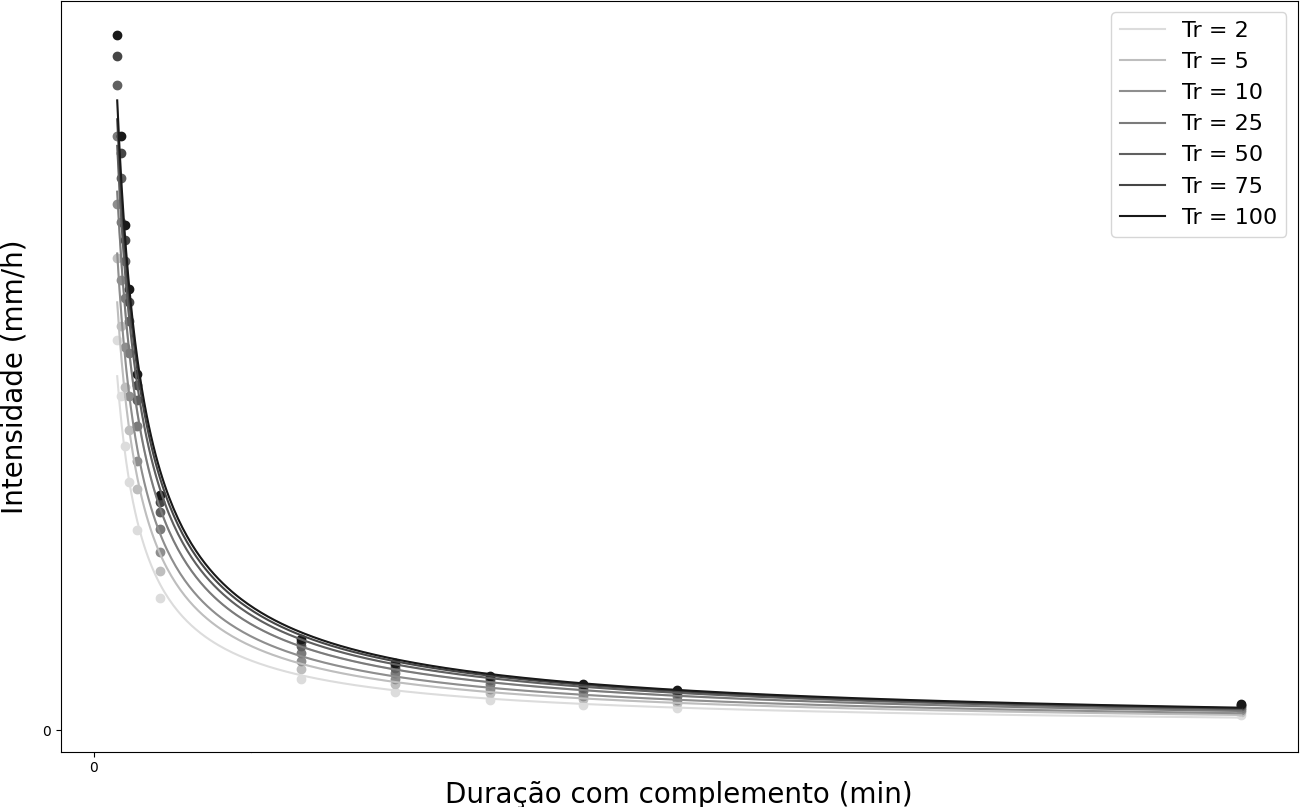
\includegraphics[width=.7325\linewidth]{figuras/curvas_idf_de_intensidade_e_duracao_com_complemento.png}
	\caption*{\textbf{Fonte:} De autoria própria (2023).}
	\label{fig:curvas_idf_de_intensidade_e_duracao_com_complemento.png}
\end{figure}

Por ilação, novas funções serão geradas para o gráfico da Figura 3.2. O processo de descoberta delas será o mesmo, utilizando as equações (3.22), (3.23), (3.24) e (3.20). O que muda neste segundo uso do MMQ são as variáveis usadas nas fórmulas citadas. Sobre elas, pode-se afirmar que $n$ continua sendo a quantidade de durações utilizadas, $x$ são os logaritmos de base dez das intensidades obtidas (3.19), e $y$ são os logaritmos de base dez das durações arbitradas com a adição do parâmetro $c$. A partir dessas informações, é possível observar um gráfico de curvas diferente na Figura 3.7.\bigskip

Um novo parâmetro da equação IDF já pode ser calculado com as informações obtidas do segundo uso do MMQ, que é o $d$ (3.29). 

\begin{equation}
d = -1 * \frac{\sum{a_1}}{n}
\end{equation}
\newline
onde:
\newline
\textit{d} é um dos parâmetros da equação da intensidade das chuvas, (adimensional);
\newline
$a_1$ é um ajuste do segundo uso do método dos mínimos quadrados, (adimensional);
\newline
\textit{n} é a quantidade total de $a_1$, (adimensional).\bigskip

Continuando com os cálculos dos parâmetros da IDF, será usado o MMQ pela terceira e última vez. Porém, a relação agora será entre o logaritmo de base dez dos tempos de retorno e os ajustes $b_2$ calculados a partir da relação da intensidade com a duração mais o parâmetro $c$. Isso resultará em uma nova relação entre os ajustes observado na sentença (3.30).\bigskip

\begin{equation}
\begin{cases}
a_1 = a_2 \\
b_1 = 10^{b_2}
\end{cases}
\end{equation}
\newline
onde:
\newline
$a_1$, $a_2$, $b_1$, $b_2$ são ajustes do método dos mínimos quadrados, (adimensional).\bigskip

Outro detalhe é que a função será traçada a partir de uma reta, com a da fórmula (3.21) para ajustes lineares, vista na Figura 3.8.\bigskip

\begin{figure}[!ht]
	\centering
	\caption{Reta da relação entre tempo de retorno e ajuste $b_2$.}
	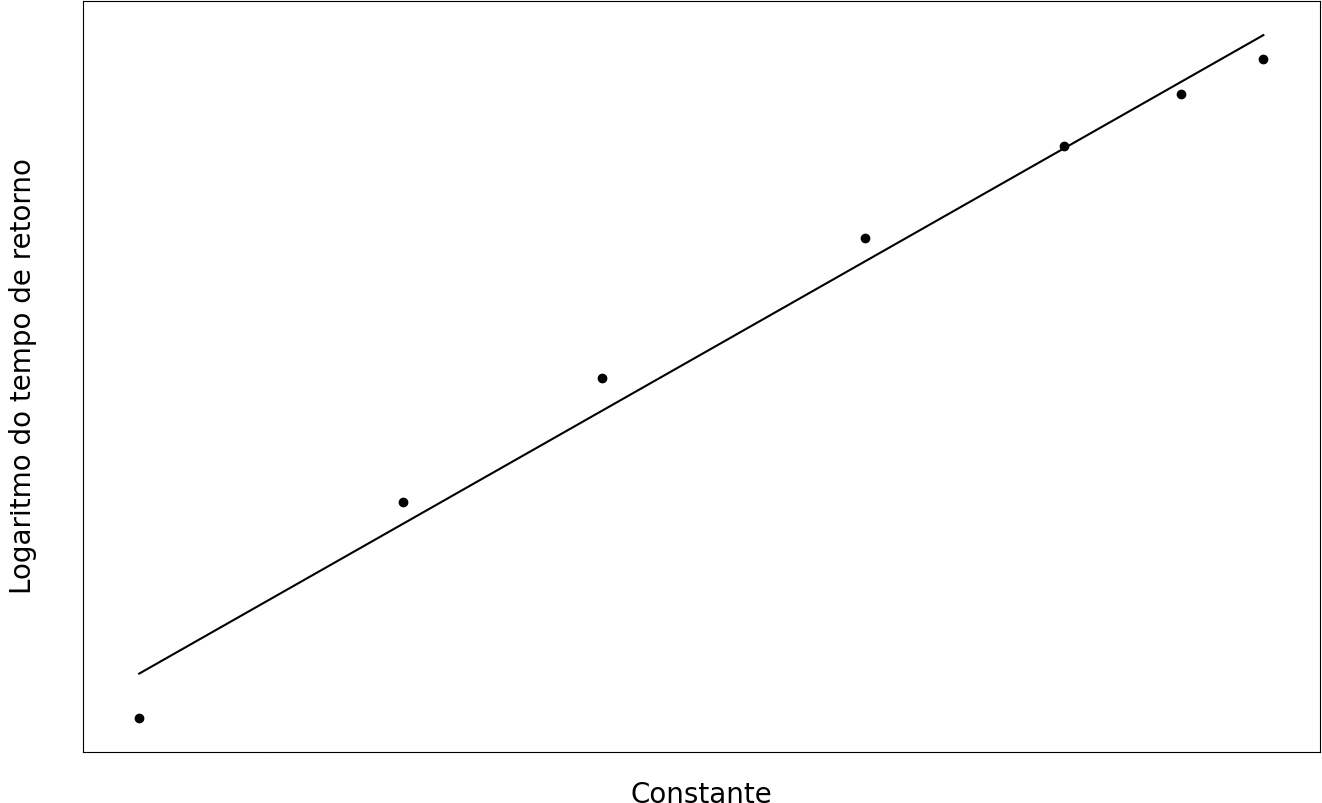
\includegraphics[width=.7325\linewidth]{figuras/reta_de_tempo_de_retorno.png}
	\caption*{\textbf{Fonte:} De autoria própria (2023).}
	\label{fig:reta_de_tempo_de_retorno.png}
\end{figure}

\newpage

Para descobrir a função da reta que pode ser vista na Figura 3.3, novamente, é importante declarar quais serão as variáveis usadas nas fórmulas (3.22) e (3.23). Pode-se dizer que $n$ será a quantidade de tempos de retorno utilizados, $x$ são os logaritmos de base dez dos tempos de retorno, e $y$ são os os ajustes $b_2$ calculados a partir da relação das intensidades com as durações mais o parâmetro $c$, no segundo uso do MMQ. As informações encontradas serão aplicadas na fórmula (3.21), após a relação entre os ajustes $a_1$ e $b_1$ feita em (3.30).

Tendo como base os ajustes da função da reta, tem-se então o necessário para descobrir os parâmetros que restam, $a$ (3.31) e $b$ (3.32), da equação IDF.\bigskip

\begin{equation}
a = b_1
\end{equation}
\newline
onde:
\newline
\textit{a} é um dos parâmetros da equação da intensidade das chuvas, (adimensional);
\newline
$b_1$ é um ajuste do terceiro uso do método dos mínimos quadrados, (adimensional).\bigskip

\begin{equation}
b = a_1
\end{equation}
\newline
onde:
\newline
\textit{b} é um dos parâmetros da equação da intensidade das chuvas, (adimensional).
\newline
$a_1$ é um ajuste do terceiro uso do método dos mínimos quadrados, (adimensional).\bigskip

Assim sendo, possui-se todos os parâmetros necessários para montar a equação IDF exposta em (3.1).

\newpage

\section{MÉTODO DO INVERSO DA POTÊNCIA DAS DISTÂNCIAS}\bigskip

O inverso da potência da distância (IDW) é uma das diversas alternativas de interpolação espacial de dados. Quando se trata de precipitações mensais e diárias, Xavier, King e Scanlon (2015), Kim e Ryu (2016) e Silva \textit{et al.} (2019) deixam claro que ele está sempre entre os métodos que apresentam os melhores resultados estatísticos em seus trabalhos. Mais adiante será apresentado de que forma seu cálculo é desenvolvido.\bigskip

\subsection{A Distância entre dois pontos}\bigskip

De início, é calculado a distância entre o ponto que se quer obter os dados de precipitação através de interpolação, e os demais que já possuem essas informações no espaço, através da fórmula da distância entre dois pontos (3.33).\bigskip

\begin{equation}
D = \sqrt{{\left(x_j - x_i\right)}^2 + {\left(y_j - y_i\right)}^2}
\end{equation}
\newline
onde:
\newline
\textit{D} é a distância entre os dois pontos, (adimensional);
\newline
$x_j$ é a latitude do ponto próximo, (adimensional);
\newline
$x_i$ é a latitude do ponto que se quer descobrir a precipitação, (adimensional);
\newline
$y_j$ é a longitude do ponto próximo, (adimensional);
\newline
$y_i$ é a longitude do ponto que se quer descobrir a precipitação, (adimensional).\bigskip

\subsection{O Inverso da potência das distâncias}\bigskip

Após descobrir às distâncias, é escolhido um dado número de pontos entre os mais próximos, e aplicar-se-á elas à formula do inverso da potência das distâncias. Assim encontra-se o peso do ponto amostral das mesmas. 

A potência a se considerar na fórmula será de número dois, que segundo Silva \textit{et al.} (2019) foi a que obteve os melhores resultados em seu trabalho. Isto porque dependendo da potência o seu comportamento muda, sendo possível analisar esta afirmação graficamente na Figura 3.9.

\newpage

\begin{figure}[!ht]
	\centering
	\caption{Potências do método do inverso da potência das distâncias}
	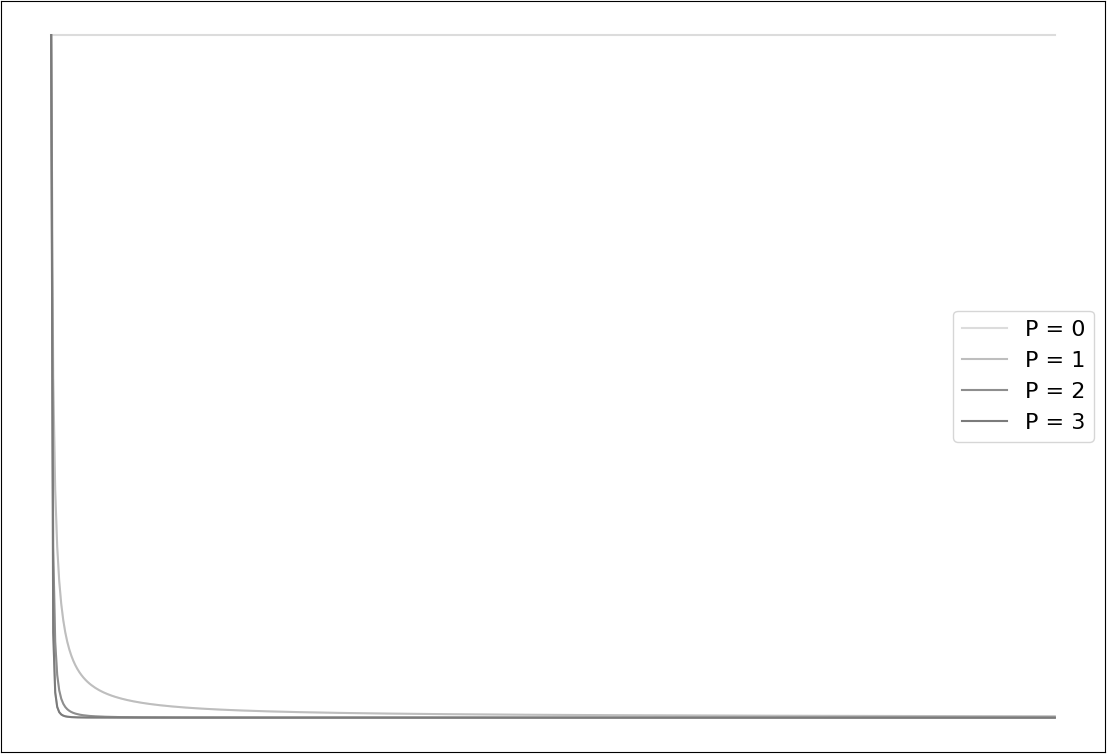
\includegraphics[width=.7325\linewidth]{figuras/potencias_da_idw.png}
	\caption*{\textbf{Fonte:} De autoria própria (2023).}
	\label{fig:potencias_da_idw.png}
\end{figure}

\begin{equation}
W = \frac{1}{D^P} = \frac{1}{D^2}
\end{equation}
\newline
onde:
\newline
\textit{W} é o peso do ponto amostral, (adimensional);
\newline
\textit{D} é a distância entre os dois pontos, (adimensional);
\newline
\textit{P} é a potência elevada da distância, (adimensional).\bigskip

\subsection{A Média ponderada das precipitações}\bigskip

Obtendo o peso do ponto amostral para cada uma das distâncias mais próximas ao ponto que se quer interpolar a precipitação, basta fazer a média ponderada das precipitações (3.35) usando seus respectivos pesos encontrados na fórmula (3.34).\bigskip

\begin{equation}
P(x_i ; y_i) = \frac{\sum{\left(P(x_j ; y_j) * W_j\right)}}{\sum{W_j}}
\end{equation}
\newline
onde:
\newline
$P(x_i ; y_i)$ é a precipitação a ser descoberta, (mm));
\newline
$P(x_j ; y_j)$ é a precipitação já existente, (mm));
\newline
$W_j$ é o peso do ponto amostral das precipitações existentes, (adimensional).\bigskip